\documentclass[t,compress,mathserif,10pt,xcolor=dvipsnames, table, aspectratio=43]{beamer}

\usepackage[T1]{fontenc}
\usepackage[utf8]{inputenc}
\usepackage[frenchb]{babel}
\usepackage{eulervm}
\usepackage{etoolbox,refcount}

%%%%% Colors
\definecolor{bleuUni}{RGB}{0, 157, 224}
\definecolor{marronUni}{RGB}{68, 58, 49}
\usecolortheme[named=bleuUni]{structure}
\input{colors}
%%%%%%%%%%%%%%%%%%%

%%%%% Tabs
\usepackage{booktabs}
\usepackage{multirow}
\usepackage{multicol}
\usepackage{makecell}
%%%%%%%%%%%%%%%%%%%%


%%%%% Plots
\usepackage{pgfplots}
 \pgfplotsset{compat=newest}
 \usepgfplotslibrary{groupplots}
\usepackage{tikz}
  \usetikzlibrary{matrix, positioning, patterns, shapes, arrows, shapes.multipart, decorations.pathmorphing}
\usepackage{circuitikz}
\usepackage{tikz-timing}      % package pour les chronogrammes
\usepackage{caption}
\usepackage{graphicx}
\usepackage[export]{adjustbox} %align in includegraphics
%%%%%%%%%%%%%%%%%%%%


%%%%% Algo
\usepackage[french,onelanguage, ruled, linesnumbered, vlined]{algorithm2e}
\SetAlFnt{\footnotesize}
%%%%%%%%%%%%%%%%%%%%


%%%%% Math
\usepackage{stmaryrd} %llbracket
\usepackage{amsmath}
\usepackage{amssymb}
\usepackage{marvosym} %grosse fleche
\usepackage{calc}
\DeclareMathOperator{\card}{card}
\DeclareMathOperator*{\maxstar}{max*}
\DeclareMathOperator*{\argmax}{arg\,max}
\DeclareMathOperator*{\decide}{decide}
\DecimalMathComma
%%%%%%%%%%%%%%%%%%%%


%%%%%% Special commands : ddfrac and actionenv and compresslist
\newcommand\ddfrac[2]{\frac{\displaystyle #1}{\displaystyle #2}}

\newenvironment<>{varblock}[2][\textwidth]{%
  \setlength{\textwidth}{#1}
  \begin{actionenv}#3%
    \def\insertblocktitle{#2}%
    \par%
    \usebeamertemplate{block begin}}
  {\par%
    \usebeamertemplate{block end}%
  \end{actionenv}}

\newcommand{\compresslist}{ % Define a command to reduce spacing within itemize/enumerate environments, this is used right after \begin{itemize} or \begin{enumerate}
\setlength{\itemsep}{1pt}
\setlength{\parskip}{0pt}
\setlength{\parsep}{0pt}
}
%%%%%%%%%%%%%%%%%%%%%%%%%


%%%%% Beamer
\usepackage[bars]{beamerthemetree} % Beamer theme v 2.2
\mode<presentation>
\newcommand*\oldmacro{}%
\let\oldmacro\insertshorttitle%
\renewcommand*\insertshorttitle{%
 \oldmacro\hfill%
\insertframenumber\,/\,\inserttotalframenumber}
\setbeamertemplate{footline}[frame number]
\setbeamersize{text margin left=10pt,text margin right=10pt}
\setbeamerfont{frametitle}{size=\small}
\setbeamertemplate{frametitle}{ \nointerlineskip %
\begin{beamercolorbox}[wd=\paperwidth,ht=2.2ex,dp=.9ex,left]{frametitle} %
                       \hspace*{2ex}\strut\bfseries\color{bleuUni!15!white}\insertframetitle\strut\par %
\end{beamercolorbox}}

%\setbeamerfont{headline}{size=\footnotesize}

% \usepackage{animate}
% \usepackage{multimedia}
\usetheme{Ilmenau} % Beamer theme v 3.0
\setbeamercolor{section in head/foot}{bg=marronUni}
\useinnertheme{circles} %rectangle bullet points instead of circle ones
\usepackage{beamerthemebars}
\beamertemplatenavigationsymbolsempty
%\setbeamercolor{navigation symbols dimmed}{fg=red!80!black}
%\setbeamercolor{navigation symbols}{fg=red!80!black}
%%%%%%%%%%%%%%%%%%%%%%%%%

\setbeamertemplate{headline}{%
\begin{beamercolorbox}[colsep=1.5pt]{upper separation line head}
\end{beamercolorbox}
\begin{beamercolorbox}{section in head/foot}
    \vskip2pt\insertsectionnavigationhorizontal{\paperwidth}{}{}\vskip2pt
\end{beamercolorbox}%
\begin{beamercolorbox}[ht=10pt]{subsection in head/foot}%
    \vskip2pt\insertsubsectionnavigationhorizontal{\paperwidth}{}{}\vskip2pt
\end{beamercolorbox}%
\begin{beamercolorbox}[colsep=1.5pt]{lower separation line head}
\end{beamercolorbox}
}


%%%%% Title
\title{\textbf{Contributions à l'amélioration des \\%
               performances de décodage des turbo codes : \\%
               algorithmes et architecture}}
%\subtitle{algorithms et arhitecture}\hspace{10.7cm}
\author[Thibaud Tonnellier\hspace{7.51cm}{thibaud.tonnellier@ims-bordeaux.fr}]    {Thibaud Tonnellier}
\titlegraphic{
\includegraphics[height=.7cm]{logos/ims.png} \hfil %
              
\includegraphics[height=.7cm]{logos/inp.PNG} \hfil %
              
\includegraphics[height=.7cm]{logos/ub.png}  \hfil %
              
\includegraphics[height=.7cm]{logos/tas.png}}
%\pgfdeclareimage[height=.8cm]{le-logo}{logo.png}
%\logo{\pgfuseimage{le-logo}\hspace{\dimexpr\paperwidth-1.55cm}\vspace{-8pt}}
%%%%%%%%%%%%%%%%%%%%%%%%%


%%%%% Contents each new sec and subsec
\AtBeginSection[]
{
  \ifnumcomp{\value{section}}{=}{1}{}{
    \begin{frame}[c]{Plan}
      \centering
      \tableofcontents[
          currentsection,
          hideothersubsections
          %subsectionstyle=show/hide
      ]
    \end{frame}
  }
}

\AtBeginSubsection[]
{
  \begin{frame}[c]{Plan}
    \tableofcontents[
      currentsection,
      sectionstyle=show/shaded,
      subsectionstyle=show/shaded/hide
    ]
  \end{frame}
}

%%%%%%%%%%%%%%%%%%%%%%%%%%%%%%%%%%%%%%%%%%%%%%%%%%%%%%%%%%%%%%%%%%%%%%%%%%%%%%%%
\begin{document}

\begin{frame}[c]
  \titlepage
\end{frame}

%%%%%%%%%%%%%%%%%%%%%%%%%%%%%%%%%%%%%%%%%%%%%%%%%%%%%%%%%%%%%%%%%%%%%%%%%%%%%%%%
\section[]{Contexte}
\begin{frame}[c]
\centering
  Slide ctx 1
\end{frame}

\begin{frame}[c]
\centering
  Slide ctx 2
\end{frame}

\begin{frame}[c]
  \tableofcontents[ 
      subsectionstyle=hide,
  ]
\end{frame}

%%%%%%%%%%%%%%%%%%%%%%%%%%%%%%%%%%%%%%%%%%%%%%%%%%%%%%%%%%%%%%%%%%%%%%%%%%%%%%%%
\section[Introduction]{Introduction et problématique} 

%%%%%%%%%%%%%%%%%%%%%%%%%%%%%%%%%%%%%%%%
\subsection{Le codage de canal}
\begin{frame}[c]{La théorie de l'information} 
\begin{itemize}\setlength\itemsep{1em}
    \item En 1948, Claude Shannon ouvre la voie à la théorie de l'information.
    \item \og Le problème de la communication est de reproduire exactement ou approximativement un message donné d'un point à un autre. \fg
    \item Première étape : dresser le modèle d'une communication.
  \end{itemize}
  \begin{center}
    \includegraphics[width=0.6\textwidth]{../main/ch1_fig/shParadigm.pdf}
  \end{center}
  \begin{itemize}
    \item Deuxième étape : envisager l'information de manière abstraite.
    \item Résultat : \og La théorie mathématique de l'information \fg 
\end{itemize}
\end{frame}

\begin{frame}[c]{La théorie de l'information : Résultats} 
\begin{itemize}\setlength\itemsep{1em}
  \item Deux théorèmes fondamentaux :
  \begin{itemize}
    \item Codage de source : obtenir le maximum de concision dans l’expression d'un message.
    \item Codage de canal : rendre robuste un message face aux perturbations du canal.    
  \end{itemize}
  \item Schéma fondamental de la communication :
  \end{itemize}
  \begin{center}
    \includegraphics[width=0.7\textwidth]{../main/ch1_fig/shParadigm2.pdf}
  \end{center}
\end{frame}

\begin{frame}[c]{La limite de Shannon}
  \begin{itemize}\setlength\itemsep{1em}
    \item \og Il existe un code de taille $N$ tel que si $R<C$ la probabilité d'erreur après décodage soit inférieure à $\epsilon$ \fg.
    \begin{itemize}
      \item N : suffisamment grand,
      \item R : rendement du code,
      \item C : capacité du canal.
    \end{itemize}
    \item Mesure de la performance d'un système de communication.
    \item Un code atteignant la \textbf{capacité du canal} peut être considéré comme \textbf{optimal}.
    \item Shannon énonce l'existence d'un tel code et non son obtention.
    \item But du codage de canal : définir des codes s'approchant \textbf{au plus près} de cette limite théorique tout en assurant un décodage \textbf{relativement simple}.
  \end{itemize}
\end{frame}

\begin{frame}[c]{Historique}
  \begin{itemize}\setlength\itemsep{1em}
    \item 1950 : code de Hamming,
    \item 1954 : codes de Reed-Muller,
    \item 1955 : codes convolutifs (P. Elias),
    \item 1959 : codes BCH,
    \item 1962 : codes LDPC (R. Gallager),
    \item 1966 : concaténation de codes (D. Forney).
  \end{itemize}
\end{frame}

\begin{frame}[c]{Courbes de performances et limites}
\begin{center}
\begin{tikzpicture}
  \begin{semilogyaxis}[footnotesize, width=0.9\linewidth, height=0.5\linewidth,    
      xmin=-1, xmax=10, xtick={-1, 0,...,10},
      ymin=2e-6,  ymax=0.11,
      xlabel=$E_b/N_0 \text{(dB)}$, 
      ylabel=\only<1>{Taux d'erreur binaire}\only<2->{Probabilité et taux d'erreurs binaires},
      grid=both, grid style={gray!30},
    tick align=outside, tickpos=left,  legend columns=2, legend style={at={(1, -.25), anchor=north}, /tikz/column 2/.style={column sep=5pt}} ]
      \only<2->{\addplot[mark=none, Paired-3, thick] coordinates {(0.187,0.000001)(0.187,0.1)};}
      \only<3->{\draw[pattern=north west lines, draw=none, pattern color=Paired-7] (axis cs:-1,1e-6)
      rectangle (axis cs:0.184, 1e-3);%
      \addlegendimage{pattern=north west lines, draw=none, pattern color=Paired-7,  area legend};}
      \only<4->{\addplot[mark=o,Paired-1, semithick]  table [x=SNR, y=BER] {../main/ch1_fig/berRSC.dat};}
      \only<5->{\addplot[mark=none,Paired-5, semithick]  table [x=SNR, y=BER] {../main/ch1_fig/berBPSK.dat}; }
      \only<6->{\addplot [<->] coordinates {(5.4, 1e-4) (8.3, 1e-4)};}
     
      \only<2->{\legend{Limite de Shannon pour R=1/2,%
                        Zone inatteignable,%
                        Décodage MAP code RSC R=1/2 $\nu = 3$,%      
                        Non codée,%
                        Gain de codage }}%à $10^{-4}$}}
  \end{semilogyaxis}
\end{tikzpicture}  
\end{center}
\end{frame} 

% \begin{frame}[c]{Définitions}
%  Performances, EF, spectre, 
% \end{frame}

%%%%%%%%%%%%%%%%%%%%%%%%%%%%%%%%%%%%%%%%
\subsection{Les turbo codes}
\begin{frame}[c]{Historique}
  \begin{itemize}
    \item Maitrise du décodage probabiliste (implantation SOVA)%, Hagenauer : 89
    \item Jusqu'alors, gain de codage : 7 dB 
    \begin{itemize}
      \item concaténation série CC + RS, entrelacement, décodage dur.
    \end{itemize} 
    \begin{center}
    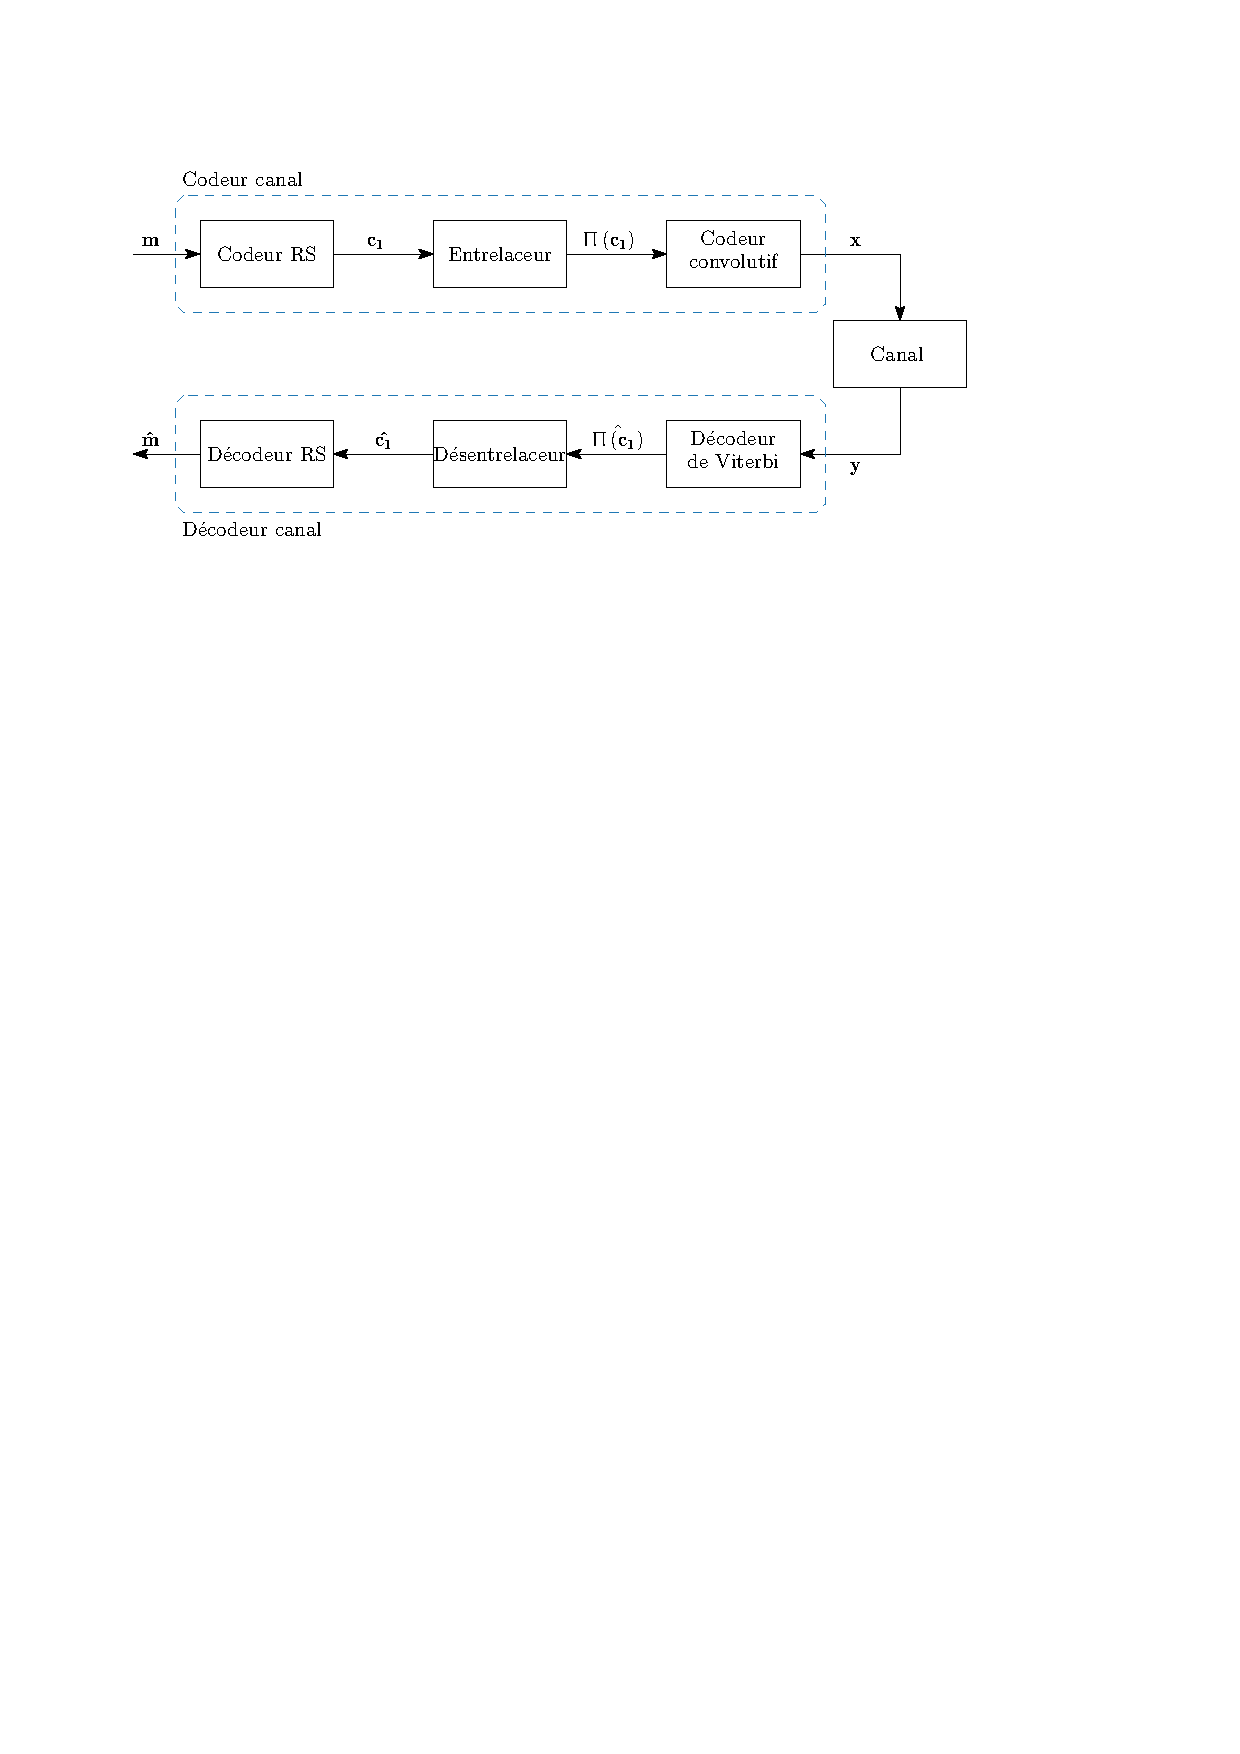
\includegraphics[width=0.7\textwidth]{../main/ch1_fig/nasa.pdf}
    \end{center}
    \item Hagenhauer et Hoeher : proposition concaténation série de CC.
    \item Berrou s’attelle a expérimenter le décodage de cette concaténation => décodage itératif
    \item Amélioration : concaténation parallèle de codeurs RSC
    \item Rupture scientifique en terme de couple performances de décodage / complexité du décodage
  \end{itemize}
\end{frame}

\begin{frame}[c]{Un codeur de turbo code convolutif parallèle}
\begin{center}
  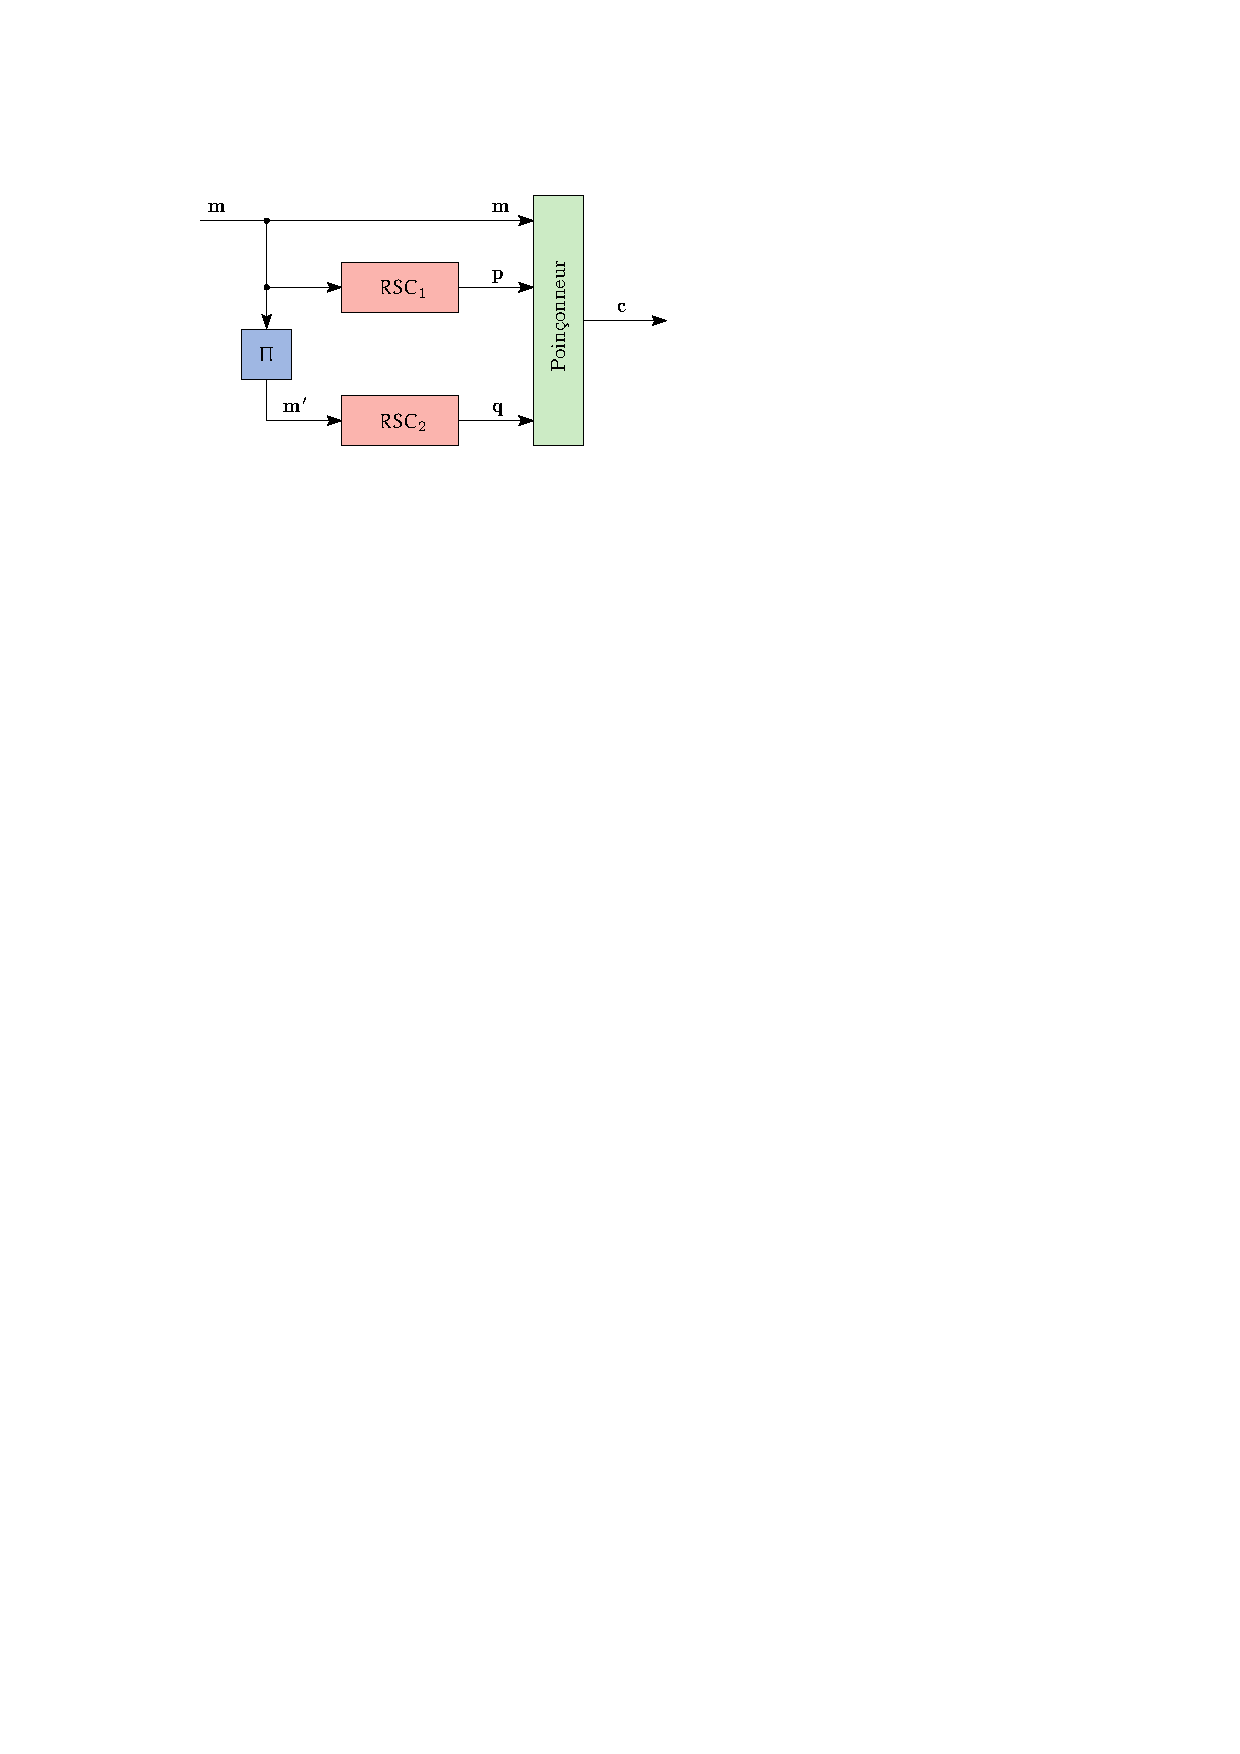
\includegraphics[width=0.7\linewidth]{../main/ch1_fig/turboEnc.pdf}
  \end{center}
\end{frame}

\begin{frame}[c]{Détail}
\begin{center}
  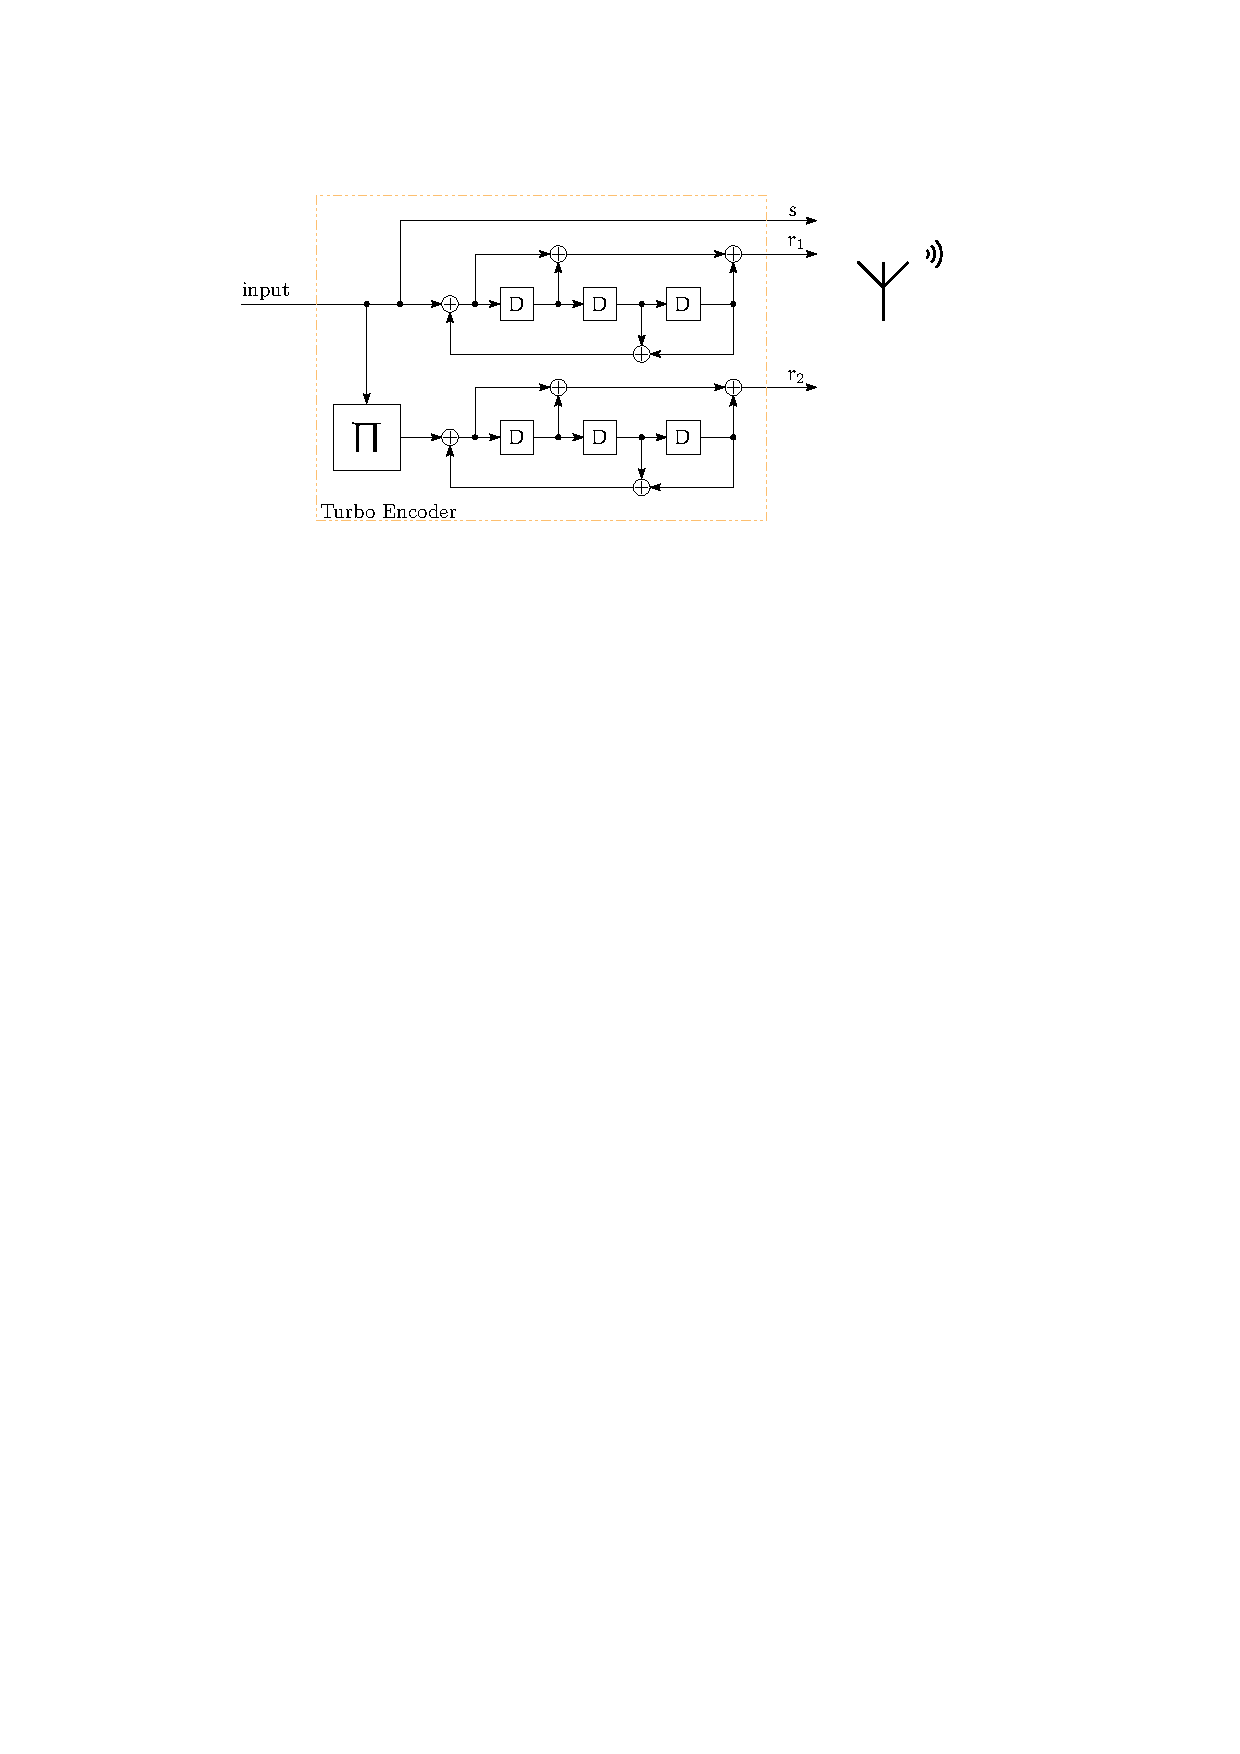
\includegraphics[width=.8\textwidth, page=1]{fig/encoder.pdf}
  \end{center}
  \begin{itemize}
    \item Ajouter treillis
  \end{itemize}
\end{frame}

\begin{frame}[c]{Retour sur la chaîne de communications numériques}
%Reprendre figure et faire aparaitre quelles données sont traitées
\begin{center}
  \includegraphics[width=.8\textwidth, page=2]{fig/shParadigm2.pdf}
\end{center}
\end{frame}

\begin{frame}[c]{Processus itératif de décodage}
%Reprendre figure et faire aparaitre quelles données sont traitées
\begin{columns}[c]
\begin{column}{0.6\textwidth}
  \begin{center}
    \only<1>{\includegraphics[width=\columnwidth, page=2]{fig/tdec.pdf}}
    \only<2>{\includegraphics[width=\columnwidth, page=3]{fig/tdec.pdf}}
    \only<3>{\includegraphics[width=\columnwidth, page=2]{fig/tdec.pdf}}
    \only<4>{\includegraphics[width=\columnwidth, page=3]{fig/tdec.pdf}}
    \only<5>{\includegraphics[width=\columnwidth, page=2]{fig/tdec.pdf}}
    \only<6>{\includegraphics[width=\columnwidth, page=3]{fig/tdec.pdf}}
    \only<7>{\includegraphics[width=\columnwidth, page=2]{fig/tdec.pdf}}
    \only<8>{\includegraphics[width=\columnwidth, page=3]{fig/tdec.pdf}}
  \end{center}
  \end{column}
\begin{column}{0.4\textwidth}
  \begin{center}
    \only<1>{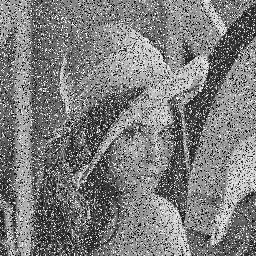
\includegraphics[width=\columnwidth]{Lenna/256/final/lena_1.png}}
    \only<2>{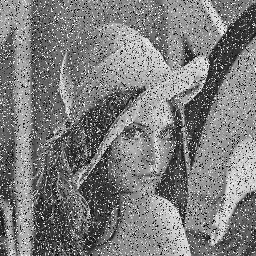
\includegraphics[width=\columnwidth]{Lenna/256/final/lena_3.png}}
    \only<3>{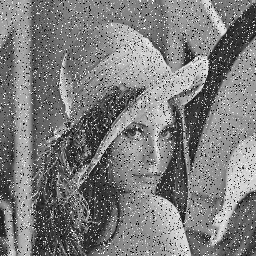
\includegraphics[width=\columnwidth]{Lenna/256/final/lena_5.png}}
    \only<4>{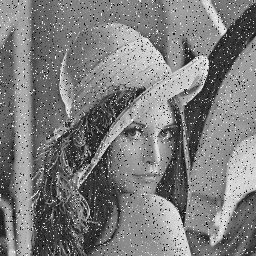
\includegraphics[width=\columnwidth]{Lenna/256/final/lena_7.png}}
    \only<5>{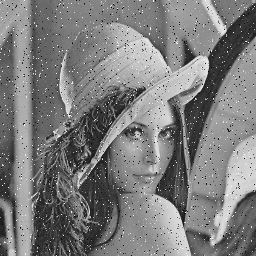
\includegraphics[width=\columnwidth]{Lenna/256/final/lena_9.png}}
    \only<6>{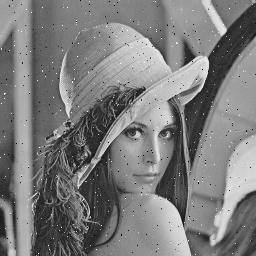
\includegraphics[width=\columnwidth]{Lenna/256/final/lena_11.png}}
    \only<7>{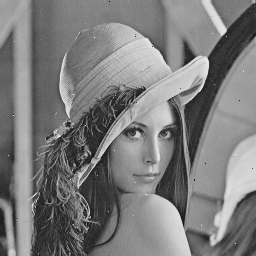
\includegraphics[width=\columnwidth]{Lenna/256/final/lena_13.png}}
    \only<8>{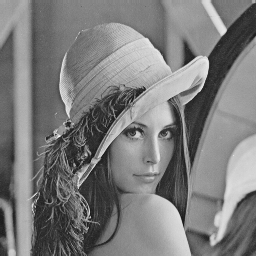
\includegraphics[width=\columnwidth]{Lenna/256/final/lena_15.png}}
  \end{center}
\end{column}
\end{columns}
\end{frame}

\begin{frame}[c]{Décodage SISO}
  \begin{itemize}\setlength\itemsep{1em}
    \item Décodage selon le treillis du code
    \item Algorithme MAP : parcours aller et retour du treillis
    \item Implantation : simplification : ML-MAP et son amélioration : EML-MAP
  \end{itemize}
\end{frame}


\begin{frame}[c]{Turbo codes doubles binaires}
  \begin{itemize}\setlength\itemsep{1em}
    \item 2 bits en entrée par codeur RSC
    \item Modification de l'algorithme MAP pour le décodage
    \item Avantages :
    \begin{itemize}
      \item Moindre poinçonnage pour de hauts rendements,
      \item Latence réduite,
      \item Plus faible dégradation entre l'algorithme MAP et ses versions simplifiées
    \end{itemize}
  \end{itemize}
\end{frame}

\begin{frame}[c]{Courbes de performances de turbo codes}
\begin{center}
  \begin{tikzpicture}
  \begin{semilogyaxis}[footnotesize, width=\linewidth, height=0.58\linewidth,    
      xmin=0.0, xmax=2.1, xtick={0,0.2,...,2.2},
      %ymin=2e-6,  ymax=0.11,
      xlabel=$E_b/N_0 \text{(dB)}$, ylabel=FER,  grid=both, grid style={gray!30},
      /pgfplots/table/ignore chars={|},
        tick align=outside, tickpos=left, legend pos=north east]
                                                                                            
                            
    \addplot[mark=o, Paired-3, semithick] table [x=Eb/N0, y=FER] {../main/ch1_fig/std/aff3ct/1784_12.txt}; 
    \addplot[mark=o, Paired-7, semithick] table [x=Eb/N0, y=FER] {../main/ch1_fig/std/aff3ct/3568_12.txt};     
    \addplot[mark=o, Paired-1, semithick] table [x=Eb/N0, y=FER] {../main/ch1_fig/std/aff3ct/1784_13.txt};
    \addplot[mark=o, Paired-5, semithick] table [x=Eb/N0, y=FER] {../main/ch1_fig/std/aff3ct/3568_13.txt}; 
                                                                                                                  
    \legend{K=1784 R=1/2,K=3568 R=1/2, K=1784 R=1/2, K=3568 R=1/3} 
  \end{semilogyaxis}
\end{tikzpicture} 
\vspace*{-1em} 
\captionof{figure}{Standard CCSDS, Canal AWGN, 10 itérations EML-MAP}
\end{center}
\end{frame}

\begin{frame}[c]{Les turbo codes standardisés étudiés}
\begin{center}
\begin{tabular}{@{}lll@{}}
\toprule
         & Binaire & Double Binaire \\ \cmidrule(l){2-2}\cmidrule(l){3-3}
8 états  & \textbf{LTE}     & \textbf{DVB-RCS}        \\
16 états & \textbf{CCSDS}   & \textbf{DVB-RCS2}       \\ \bottomrule
\end{tabular}
\end{center}
\end{frame}

\begin{frame}[c]{Performances asymptotique}
\begin{itemize}\setlength\itemsep{1em}
  \item Possibilité de prédire les performances asymptotiques de codes.
  \item Sur canal BI-AWGN, borne de l'union : 
\begin{equation*} \label{eq:uboundfer}
  P_{e,\text{ trame}} \leq \sum\limits_d A_d Q\left(\sqrt{\frac{2dRE_b}{N_0}}\right)
\end{equation*}
  \item Obtention du spectre de distance ($d,A_d, W_d$) pour calculer cette borne.
  \item Prédiction du plancher d'erreurs
\end{itemize}
\end{frame}

\begin{frame}[c]{Visualisation du plancher d'erreurs}
\begin{center}
  \begin{tikzpicture}
  \begin{semilogyaxis}[footnotesize, width=\linewidth, height=0.58\linewidth,
      xmin=0, xmax=3, xtick={0,0.4,...,3.0},
      %ymin=2e-6,  ymax=0.11,
      xlabel=$E_b/N_0 \text{(dB)}$, ylabel=FER,  grid=both, grid style={gray!30},
    tick align=outside, tickpos=left, legend pos=north east]
                                                                            
    \addplot[mark=o,Paired-1]  table [x=SNR, y=FER] {../main/ch1_fig/std/lte13_528.dat}; 
    \addplot[mark=square,Paired-5]  table [x=SNR, y=FER] {../main/ch1_fig/std/lte13_2048.dat}; 
    \addplot[mark=triangle,Paired-7]  table [x=SNR, y=FER2] {../main/ch1_fig/std/lte13_6144.dat}; 
                            
    \addplot[Paired-2]  table [x=SNR, y=FER] {../main/ch1_fig/std/lte13_528_ubound.dat}; 
    \addplot[Paired-6]  table [x=SNR, y=FER] {../main/ch1_fig/std/lte13_2048_ubound.dat}; 
    \addplot[Paired-8]  table [x=SNR, y=FER] {../main/ch1_fig/std/lte13_6144_bound.dat};                                                   
                                                                                                
    \legend{K=528, K=2048, K=6144}
                                                                                                
  \end{semilogyaxis}
\end{tikzpicture}
\vspace*{-1em} 
\captionof{figure}{Standard LTE, R=1/3, Canal AWGN, 8 itérations EML-MAP, borne de l'union}
\end{center}
\end{frame}

\begin{frame}[c]{Les causes du plancher d'erreurs}
  \begin{itemize}\setlength\itemsep{1em}
    \item Lien direct avec la distance minimale du code
   \begin{equation*}
     P_{e,\text{ trame}} \sim A_{d_{min}} Q\left(\sqrt{\frac{2d_{min}RE_b}{N_0}}\right)
   \end{equation*}
   \item Erreurs résiduelles : le mot erroné est très proche de mot transmis
\end{itemize}
\end{frame}

\begin{frame}[c]{État de l'art sur la réduction du plancher d'erreur}
  \begin{itemize}\setlength\itemsep{1em}
    \item Modification du codeur turbo :
    \begin{itemize}\setlength\itemsep{1.5ex}
      \item Augmentation du nombre d'états
      \item Amélioration entrelaceur
    \end{itemize}
    \item Concaténation de code
    \begin{itemize}\setlength\itemsep{1.5ex}
      \item BCH
      \item Code RSC de rendement 1 
      \item Code CRC
      \begin{itemize}
        \item Décodage par liste
        \item Décodage OSD
        \item Multiple turbo décodages
      \end{itemize}
    \end{itemize}
  \end{itemize}

\end{frame}

%%%%%%%%%%%%%%%%%%%%%%%%%%%%%%%%%%%%%%%%
\subsection{Conclusion et problématique}
\begin{frame}[c]{Conclusion}
\begin{itemize}\setlength\itemsep{2em}
  \item Notions de codage de canal
  \item Construction et décodage des turbo codes convolutifs
  \item Problème du plancher d'erreurs
\end{itemize}
\end{frame}

\begin{frame}[c]{Problématique}
  \begin{itemize}\setlength\itemsep{2em}
    \item Proposer une amélioration des performances de décodage des turbo codes
    \item Sans modifier le schéma de codage, pour être adapté aux turbo codes standardisés
  \end{itemize}
\end{frame}


%%%%%%%%%%%%%%%%%%%%%%%%%%%%%%%%%%%%%%%%%%%%%%%%%%%%%%%%%%%%%%%%%%%%%%%%%%%%%%%%
\section[Oscillations]{Exploitation des oscillations au cours du processus itératif de décodage}
%%%%%%%%%%%%%%%%%%%%%%%%%%%%%%%%%%%%%%%%

\subsection{Observations}
\begin{frame}[c]{Objectif}
  \begin{itemize}
    \item Exploiter de nouvelles métriques pour améliorer le décodage
    \item Études des oscillations lors du processus décodage
  \end{itemize}
  \begin{center}
  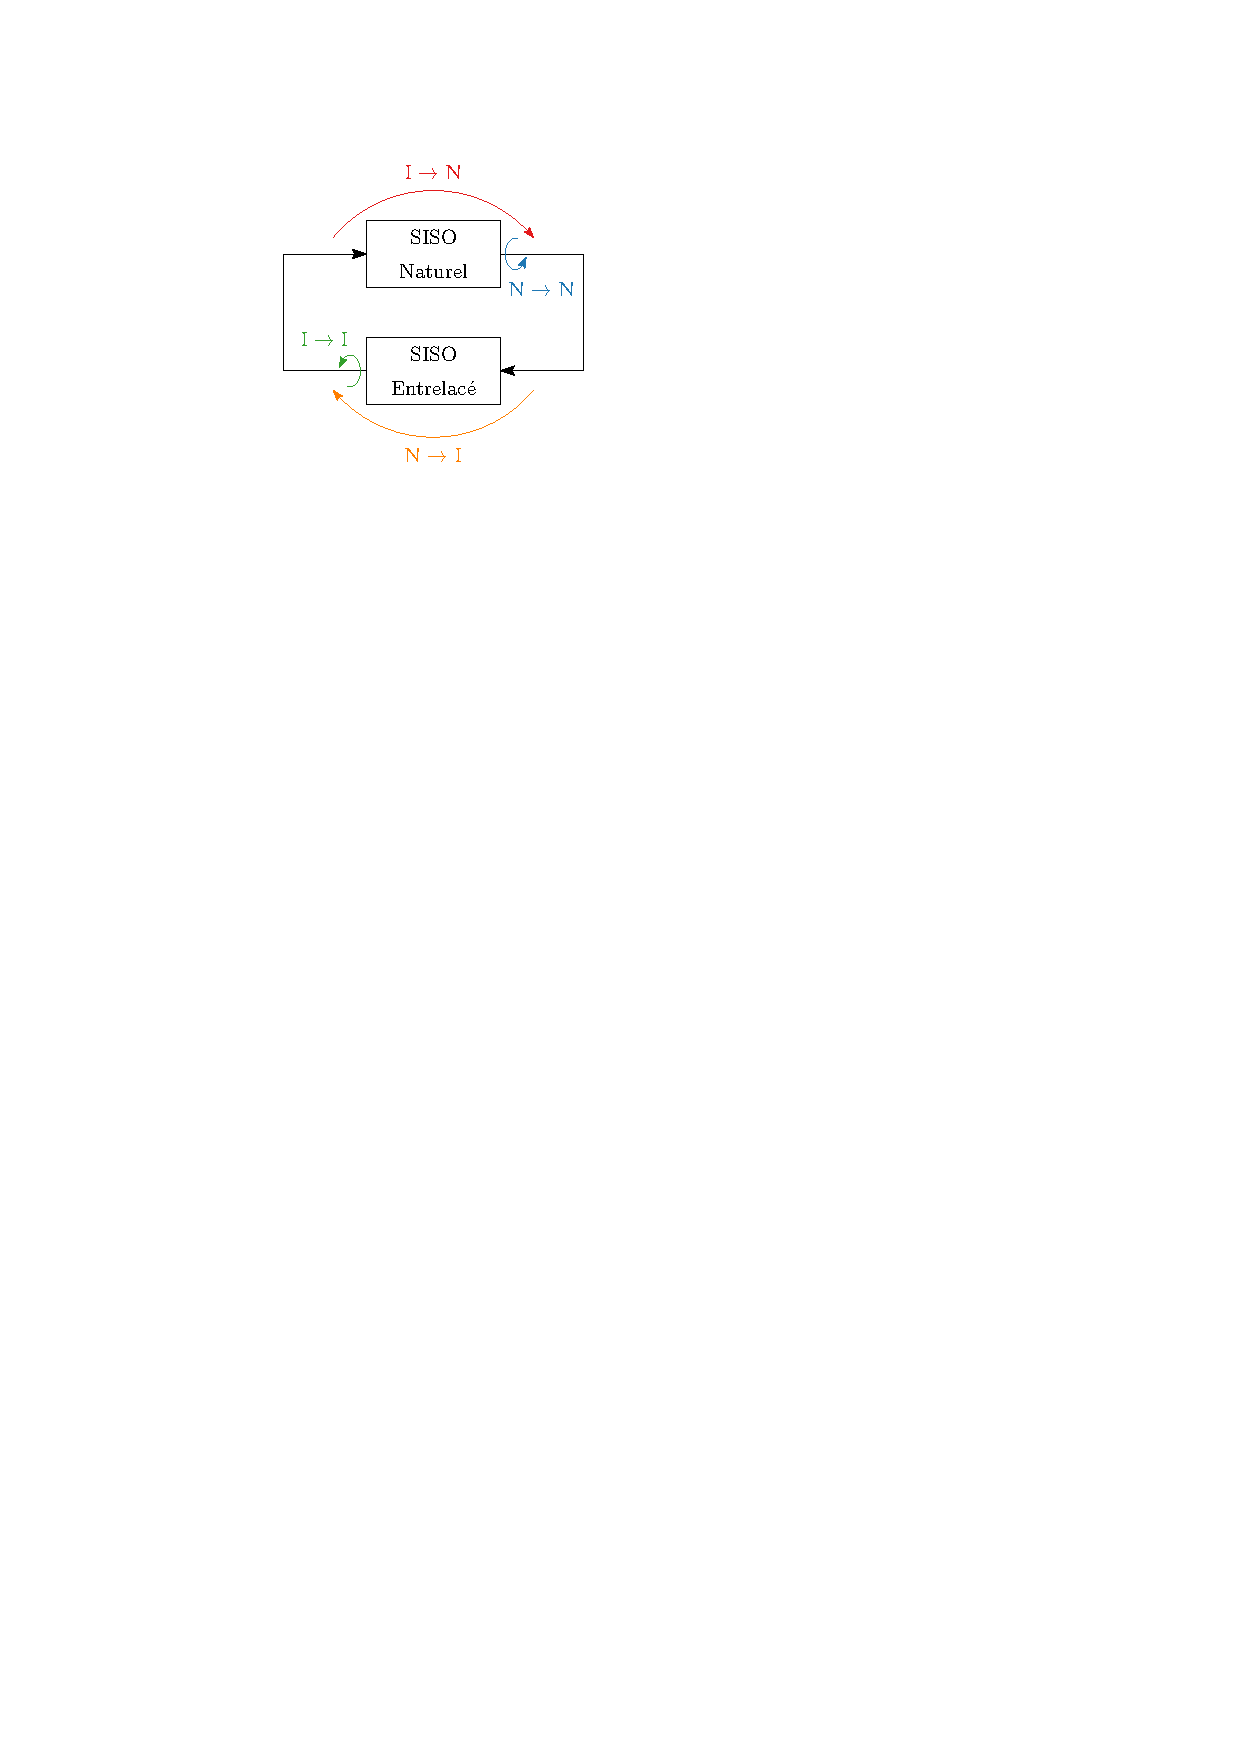
\includegraphics[width=.45\columnwidth]{../main/ch2_fig/ipe/osc.pdf}
  \end{center}
  \captionof{figure}{Les différents types d'oscillations possibles pour l'information extrinsèque.}  
\end{frame}

\begin{frame}[c]{Statistiques (1/3)}
  \begin{center}
  \includegraphics[width=.7\textwidth]{../main/ch2_fig/tikz/m_lte.pdf}
    \end{center}
  \captionof{figure}{Nombre moyen d'oscillations pour différents taux d'erreurs trame cibles, turbo code du standard LTE (K=1024, R=1/3).}
\end{frame}

\begin{frame}[c]{Statistiques (2/3)}
  Chevelures ?
\end{frame}

\begin{frame}[c]{Statistiques (3/3)}
  Distribution ?
\end{frame}

\begin{frame}[c]{Analyse}
  \begin{enumerate}
    \item Si des oscillations surviennent lors d'une itération, alors la trame n'est pas encore 
    corrigée. 
    \item Une corrélation forte entre le nombre d'erreurs et le nombre d'oscillations existe. 
    \item Si un bit oscille fortement lors du processus de décodage, alors, relativement aux autres, il a plus de chance d'être erroné.
    \item Ainsi, c'est parmi les bits oscillant le plus que se trouve la plupart des bits erronés.
    \item Cependant, comme les bits corrigés à l'issu du processus itératif oscillent eux aussi et sont majoritaires dans la 
    trame, le nombre d'oscillations ne permet pas de prédire de manière fiable si un bit est erroné.
  \end{enumerate}
\end{frame}
%%%%%%%%%%%%%%%%%%%%%%%%%%%%%%%%%%%%%%%%
\subsection{Algorithme Self-Corrected}
\begin{frame}[c]{Introduction}
  \begin{itemize}
    \item Adaptation d'une approche originellement développée pour les codes LDPC
    \item Principe : 
    \begin{enumerate}
      \item Détecter les messages non fiables échangés entre les nœuds de variable et de parité
      \item Annuler la contribution d'un nœud de variable à un nœud de parité
    \end{enumerate}
    \item Algorithme
    \begin{itemize}
      \item La contribution d’un nœud de variable au nœud de parité est effacée si son signe a changé par rapport à
l’itération précédente.
      \item Sinon elle  est transmise sans modification
    \end{itemize}
  \end{itemize}
\end{frame}

\begin{frame}[c]{Adaptation aux turbo codes - Principe}
\begin{itemize}\setlength\itemsep{1em}
  \item Les messages transmis entre les nœuds de parité et de variable correspondent aux informations extrinsèques
  \item L’annulation de la contribution peut être effectué lors d'un changement de signe de cette info. extrinsèque entre 2 itérations.
  \item Il ne faut pas appliquer cette correction dès le début du processus itératif 
\end{itemize}
\end{frame}

\begin{frame}[c]{Adaptation aux turbo codes - Algorithme}
\begin{center}
%\vspace*{-2ex}
\begin{minipage}{.6\textwidth}
  \begin{algorithm}[H]
    \DontPrintSemicolon
    \SetKwFunction{DA}{Décodage SISO$_1$ EML-MAP}
    \SetKwFunction{DB}{Décodage SISO$_2$ EML-MAP}  
    \For{j: 1 à  $I_{max}$}
    {
      \DA\;
      \If{j>4}
      {
        \ForEach{$k \in K$}{%
          \If{$sgn\left(\mathbf{L_{12}^{\texttt{e}\ (j)}}(k)\right) \neq sgn\left(\mathbf{L_{12}^{\texttt{e}\ (j-1)}}(k)\right)$}
          {
            {$\mathbf{L_{12}^{\texttt{e}\ (j)}}(k)\gets 0$}
          }
        }
      }
      \DB\;
      \If{j>4}
      {
        \ForEach{$k \in K$}{%
          \If{$sgn\left(\mathbf{L_{21}^{\texttt{e}\ (j)}}(k)\right) \neq sgn\left(\mathbf{L_{21}^{\texttt{e}\ (j-1)}}(k)\right)$}
          {
            {$\mathbf{L_{21}^{\texttt{e}\ (j)}}(k)\gets 0$}
          }
        }
      }
    }
  \caption{Self-Corrected EML-MAP.}
  \end{algorithm}
\end{minipage}
\end{center}
\let\thefootnote\relax\footnotetext{Extension du principe Self-Corrected de l'information extrinsèque au décodage itératif de Turbo Codes - GRETSI 2015}
\end{frame}

\begin{frame}[c]{Adaptation aux turbo codes - Performances de décodage}
  \begin{center}
    \includegraphics[width=.8\textwidth]{../main/ch2_fig/tikz/ccsds_sc.pdf}
  \end{center}
  \vspace*{-1em}
  \captionof{figure}{Comparaison des performances décodage entre les algorithme EML-MAP, SC EML-MAP et MAP. Turbo code du standard CCSDS (K=1784, R=1/3).}
\end{frame}
\begin{frame}[c]{Conclusion}
\begin{itemize}\setlength\itemsep{1em}
  \item Gains d'un ordre de grandeur en terme de FER dans la zone de convergence
  \item Conditions : 
  \begin{itemize}
    \item Nombre d'états $> 8$
    \item Itérations $> 16$ 
  \end{itemize}
  \item Simple à mettre en œuvre
  \item Pas d'adaptation trouvée pour les turbo codes doubles binaires
\end{itemize}
\end{frame}

%%%%%%%%%%%%%%%%%%%%%%%%%%%%%%%%%%%%%%%%
\subsection{Conclusion}

\begin{frame}[c]{Conclusions sur les oscillations}
\begin{itemize}\setlength\itemsep{1em}
  \item Observation de fortes corrélations entre des oscillations et des erreurs,
  \item Mais pas d'implication oscillations {\color{bleuUni}\Large\MVRightarrow} erreurs
  \item Proposition Self-Corrected
  \item Tentatives multiples décodages non fructifié
\end{itemize}
\end{frame}

%%%%%%%%%%%%%%%%%%%%%%%%%%%%%%%%%%%%%%%%%%%%%%%%%%%%%%%%%%%%%%%%%%%%%%%%%%%%%%%%
\section[Erreurs résiduelles]{Erreurs résiduelles : identification et correction}
%%%%%%%%%%%%%%%%%%%%%%%%%%%%%%%%%%%%%%%%
\subsection{Observations}
\begin{frame}[c]{Introduction}
  \begin{itemize}\setlength\itemsep{1em}
    \item Dans la zone de convergence, de nombreuses erreurs sont présentes à l’issu du décodage. 
    \item En revanche, dans la zone du plancher d’erreurs, le nombre moyen d’erreurs binaires par trame erronée est inférieur à 10. 
    \item La zone du plancher d'erreur émane de la présence \emph{d'erreurs résiduelles}
    \item Le nombre d'erreurs binaires par trame peut être caractérisé grâce au spectre de distance
  \end{itemize}
\end{frame}

\begin{frame}[c]{Exemple standard LTE}
  %\includegraphics[width=.95\textwidth, trim={0 195 0 190}, clip]{../main/ch3_fig/be/tikz/be.pdf}
  \resizebox*{\textwidth}{!}{
  \begin{tikzpicture}
    \begin{groupplot}[group style={group name=be, group size= 2 by 1, horizontal sep=1cm, vertical sep=2.5cm}, 
          height=0.6\textwidth,  width=1.1\textwidth,
          grid=both, grid style={gray!30},
          %colorbrewer cycle list=Spectral,
          ybar interval=1pt, %/pgf/bar width=3pt,
          xmin=1, xmax=22, xtick={1,2,...,22}, ymin=0,  ytick={0,10,...,45}, ymax=45, 
          grid=both, grid style={dashed, gray!50},  legend style={at={(0.5,1.03)},anchor=south},legend columns=4,
          xticklabels={1,2,3,4,5,6,7,8,9,10,11,12,13,14,15,16,17,18,19,20,>20},
          x tick label style={shift={(axis cs:1.25,0)},anchor=east,rotate=60},
          restrict y to domain*=0:45, % Cut values off at 14
          visualization depends on=rawy\as\rawy, % Save the unclipped values
          after end axis/.code={ % Draw line indicating break
            \draw [ultra thick, white, decoration={snake, amplitude=1pt}, decorate] (rel axis cs:0,0.95) -- (rel axis cs:1,0.95);
          },
          axis lines*=left,
          clip=false
          ]
   
         \nextgroupplot[ylabel=FdM (\%), legend entries = {0.9dB, 1.1dB, 1.3dB}]
         \addplot[draw=Paired-1, fill=Paired-1!50, postaction={pattern color = black!80,pattern=north west lines}] table [x=X, y expr=\thisrowno{5}/5] {../main/ch3_fig/be/dat/2048.dat};
         \addplot[draw=Paired-3, fill=Paired-3!50, postaction={pattern color = black!80,pattern=north east lines}] table [x=X, y expr=\thisrowno{6}/5] {../main/ch3_fig/be/dat/2048.dat};
         \addplot[draw=Paired-5, fill=Paired-5!50, postaction={pattern color = black!80,pattern=crosshatch dots }] table [x=X, y expr=\thisrowno{7}/5] {../main/ch3_fig/be/dat/2048.dat};
         \addplot[mark=*, only marks, black, mark options={scale=0.9, fill=Dark2-2!50 }, update limits=false] table[x=X, y=l2048] {../main/ch3_fig/be/dat/th};

         \nextgroupplot[legend entries = {0.4dB, 0.6dB, 0.8dB}]
         \addplot[draw=Paired-1, fill=Paired-1!50, postaction={pattern color = black!80,pattern=north west lines}] table [x=X, y expr=\thisrowno{3}/5] {../main/ch3_fig/be/dat/6144.dat};
         \addplot[draw=Paired-3, fill=Paired-3!50, postaction={pattern color = black!80,pattern=north east lines}] table [x=X, y expr=\thisrowno{4}/5] {../main/ch3_fig/be/dat/6144.dat};
         \addplot[draw=Paired-5, fill=Paired-5!50, postaction={pattern color = black!80,pattern=crosshatch dots }] table [x=X, y expr=\thisrowno{5}/5] {../main/ch3_fig/be/dat/6144.dat};
         \node[rotate=60] at ($(axis cs:22.1,49)+(0,0)$) {\small \textcolor{Paired-1}{53}};
         \node[rotate=60] at ($(axis cs:3.75,49)+(0,0)$) {\small \textcolor{Paired-5}{64}};
         \addplot[mark=*, only marks, black, mark options={scale=0.9, fill=Dark2-2!50 }, update limits=false] table[x=X, y=l6144] {../main/ch3_fig/be/dat/th};
         \addplot [<-, black, very thin, sharp plot, update limits=false] coordinates{(2.95,60) (3.4,60)} node [right] {{\footnotesize $76$}};        
    \end{groupplot}
        \node[below = 0.8cm of be c1r1.south] {(a) : LTE K=2048 - R=1/3};
        \node[below = 0.8cm of be c2r1.south] {(b) : LTE K=6144 - R=1/3};
  \end{tikzpicture}}
  \captionof{figure}{Distribution du nombre d’erreurs binaires. Turbo codes LTE. Décodage EML-MAP itérant 8 fois.}
\end{frame}

%%%%%%%%%%%%%%%%%%%%%%%%%%%%%%%%%%%%%%%%
\subsection{Critères d'identifications de positions erronés}
\begin{frame}[c]{Le critère}
\begin{itemize}\setlength\itemsep{2em}
  \item Suite à une étude : 
  \begin{equation*}
    \Delta(k) = |L^a(k)|, \qquad \text{avec k~}\in \llbracket0;~K \rrbracket 
  \end{equation*}
  \item Module de l'information \textit{a posteriori} {\color{bleuUni}\Large\MVRightarrow} niveau de confiance associé à chaque bit du
mot décodé.
\end{itemize}
\end{frame}

\begin{frame}[c]{Résultats d'identification}
  \resizebox*{\textwidth}{!}{
  \begin{tikzpicture}
    \begin{groupplot}[group style={group name=be, group size= 2 by 1, horizontal sep=1cm, vertical sep=3cm}, 
          height=0.5\textwidth,  width=.7\textwidth,
          grid=both, grid style={gray!30},
          %colorbrewer cycle list=Spectral,
          ybar interval = 1pt, /pgf/bar width=-5pt,
          xmin=1, xmax=6, ymin=0,  ytick={0,10,...,105}, ymax=105, 
          grid=both, grid style={dashed, gray!50},  legend style={at={(0.5,1.05)},anchor=south},legend columns=4,
          xticklabels={4, 6, 8, 10, 20},
          x tick label style={shift={(axis cs:1.15,-2.5)},anchor=east},  
          axis lines*=left,
          xlabel=Profondeur de recherche,
          legend entries = {Métrique $\Delta$}
          %legend entries = {Métrique Apost.~~, Métrique Ext.~~}
          ]
         
      \nextgroupplot[ylabel=Identification réussie (\%),]
        \only<1>{\addplot[draw=marronUni!50!black, fill=bleuUni!50] table [x=X, y expr=\thisrowno{2}/5.0] {../main/ch3_fig/id2/dat/2048};}
                 %\addplot[draw=Paired-1, fill=Paired-1!50, postaction={pattern color = black!80,pattern=north west lines}] table [x=X, y expr=\thisrowno{1}/5.0] {../main/ch3_fig/id2/dat/2048};}

        \only<2>{\addplot[draw=marronUni!50!black, fill=bleuUni!50] table [x=X, y expr=\thisrowno{4}/5.0] {../main/ch3_fig/id2/dat/2048};}
                 %\addplot[draw=Paired-1, fill=Paired-1!50, postaction={pattern color = black!80,pattern=north west lines}] table [x=X, y expr=\thisrowno{3}/5.0] {../main/ch3_fig/id2/dat/2048};}

        \only<3>{\addplot[draw=marronUni!50!black, fill=bleuUni!50] table [x=X, y expr=\thisrowno{6}/5.0] {../main/ch3_fig/id2/dat/2048};}
                 %\addplot[draw=Paired-1, fill=Paired-1!50, postaction={pattern color = black!80,pattern=north west lines}] table [x=X, y expr=\thisrowno{5}/5.0] {../main/ch3_fig/id2/dat/2048};}

      \nextgroupplot[]
        \only<1>{\addplot[draw=marronUni!50!black, fill=bleuUni!50] table [x=X, y expr=\thisrowno{2}/5.34] {../main/ch3_fig/id2/dat/6144};}
                 %\addplot[draw=Paired-1, fill=Paired-1!50, postaction={pattern color = black!80,pattern=north west lines}] table [x=X, y expr=\thisrowno{1}/5.34] {../main/ch3_fig/id2/dat/6144};}

        \only<2>{\addplot[draw=marronUni!50!black, fill=bleuUni!50] table [x=X, y expr=\thisrowno{4}/5.00] {../main/ch3_fig/id2/dat/6144};}
                 %\addplot[draw=Paired-1, fill=Paired-1!50, postaction={pattern color = black!80,pattern=north west lines}] table [x=X, y expr=\thisrowno{3}/5.00] {../main/ch3_fig/id2/dat/6144};}

        \only<3>{\addplot[draw=marronUni!50!black, fill=bleuUni!50] table [x=X, y expr=\thisrowno{6}/5.00] {../main/ch3_fig/id2/dat/6144};}
                 %\addplot[draw=Paired-1, fill=Paired-1!50, postaction={pattern color = black!80,pattern=north west lines}] table [x=X, y expr=\thisrowno{5}/5.00] {../main/ch3_fig/id2/dat/6144};}     
    \end{groupplot}
    \only<1>{\node[below = 1cm of be c1r1.south] {(a) : LTE K=2048, SNR=0.9dB (TET=$1.3\times 10^{-4}$)};}
    \only<2>{\node[below = 1cm of be c1r1.south] {(a) : LTE K=2048, SNR=1.1dB (TET=$1.0\times 10^{-5}$)};}
    \only<3>{\node[below = 1cm of be c1r1.south] {(a) : LTE K=2048, SNR=1.3dB (TET=$4.3\times 10^{-6}$)};}
    \only<1>{\node[below = 1cm of be c2r1.south] {(b) : LTE K=6144, SNR=0.4dB (TET=$1.4\times 10^{-1}$)};}
    \only<2>{\node[below = 1cm of be c2r1.south] {(b) : LTE K=6144, SNR=0.6dB (TET=$1.3\times 10^{-3}$)};}
    \only<3>{\node[below = 1cm of be c2r1.south] {(b) : LTE K=6144, SNR=0.8dB (TET=$3.4\times 10^{-5}$)};}
  \end{tikzpicture}}
  \captionof{figure}{Pourcentage d’identification réussie des erreurs résiduelles. Turbo codes du standard LTE. Décodage EML-MAP itérant 8 fois.}
\end{frame}

\begin{frame}[c]{Le critère pour les turbo codes double binaires}
\begin{itemize}\setlength\itemsep{2em}
  \item Considérer uniquement les deux symboles les plus probables : 
  \begin{equation*} \begin{split}
  {\quad \color{bleuUni}\bullet}\quad S_{M_x}(k) = \argmax\limits_{s\in\llbracket0;3\rrbracket}\left(l^a_s(k)\right)
  \end{split}\qquad
  \begin{split}
   {\color{bleuUni}\bullet}\quad S_{M_y}(k) = \argmax\limits_{s\in\llbracket0;3\rrbracket\setminus{S_{M_x}(k)}}\left(l^a_s(k)\right)
  \end{split} 
\end{equation*}
\begin{equation*}
  \Delta(k) = l^a_{S_{M_x}}(k)-l^a_{S_{M_y}}(k)
\end{equation*}
\item Permet de me calculer qu'une distance par symbole
\end{itemize}
\end{frame}

\begin{frame}[c]{Résultats d'identification}
  \resizebox*{\textwidth}{!}{
  \begin{tikzpicture}
    \begin{groupplot}[group style={group name=be, group size= 2 by 1, horizontal sep=1cm, vertical sep=3cm}, 
          height=0.5\textwidth,  width=.7\textwidth,
          grid=both, grid style={gray!30},
          %colorbrewer cycle list=Spectral,
          ybar interval,% = -1pt, /pgf/bar width=-5pt,
          xmin=1, xmax=6, ymin=0,  ytick={0,10,...,105}, ymax=105, 
          grid=both, grid style={dashed, gray!50},  legend style={at={(0.5,1.05)},anchor=south},legend columns=4,
          xticklabels={4, 6, 8, 10, 20},
          x tick label style={shift={(axis cs:1.15,-2.5)},anchor=east},  
          axis lines*=left,
          xlabel=Profondeur de recherche,
          legend entries = {Métrique $\Delta$}
          %legend entries = {Métrique Apost.~~, Métrique Ext.~~}
          ]
        
       \nextgroupplot[ylabel=Identification réussie (\%),]
         \only<1>{\addplot[draw=marronUni!50!black, fill=bleuUni!50] table [x=X, y expr=\thisrowno{2}] {../main/ch3_fig/id2/dvb/dat/752_13};}
                 %\addplot[draw=Paired-1, fill=Paired-1!50, postaction={pattern color = black!80,pattern=north west lines}] table [x=X, y expr=\thisrowno{1}/5.0] {../main/ch3_fig/id2/dvb/dat/752_};}

        \only<2>{\addplot[draw=marronUni!50!black, fill=bleuUni!50] table [x=X, y expr=\thisrowno{4}] {../main/ch3_fig/id2/dvb/dat/752_13};}
                 %\addplot[draw=Paired-1, fill=Paired-1!50, postaction={pattern color = black!80,pattern=north west lines}] table [x=X, y expr=\thisrowno{3}/5.0] {../main/ch3_fig/id2/dvb/dat/752_};}

        \only<3>{\addplot[draw=marronUni!50!black, fill=bleuUni!50] table [x=X, y expr=\thisrowno{6}] {../main/ch3_fig/id2/dvb/dat/752_13};}
                 %\addplot[draw=Paired-1, fill=Paired-1!50, postaction={pattern color = black!80,pattern=north west lines}] table [x=X, y expr=\thisrowno{5}/5.0] {../main/ch3_fig/id2/dvb/dat/752_};}

      \nextgroupplot[]
        \only<1>{\addplot[draw=marronUni!50!black, fill=bleuUni!50] table [x=X, y expr=\thisrowno{2}] {../main/ch3_fig/id2/dvb/dat/752_67};}
                 %\addplot[draw=Paired-1, fill=Paired-1!50, postaction={pattern color = black!80,pattern=north west lines}] table [x=X, y expr=\thisrowno{1}/5.34] {../main/ch3_fig/id2/dvb/dat/752_};}

        \only<2>{\addplot[draw=marronUni!50!black, fill=bleuUni!50] table [x=X, y expr=\thisrowno{4}] {../main/ch3_fig/id2/dvb/dat/752_67};}
                 %\addplot[draw=Paired-1, fill=Paired-1!50, postaction={pattern color = black!80,pattern=north west lines}] table [x=X, y expr=\thisrowno{3}/5.00] {../main/ch3_fig/id2/dvb/dat/752_};}

        \only<3>{\addplot[draw=marronUni!50!black, fill=bleuUni!50] table [x=X, y expr=\thisrowno{6}] {../main/ch3_fig/id2/dvb/dat/752_67};}
                 %\addplot[draw=Paired-1, fill=Paired-1!50, postaction={pattern color = black!80,pattern=north west lines}] table [x=X, y expr=\thisrowno{5}/5.00] {../main/ch3_fig/id2/dat/6144};}     
     \end{groupplot}
    \only<1>{\node[below = 1cm of be c1r1.south] {(a) : DVB-RCS K=752, R=1/3, SNR=1.0dB};}
    \only<2>{\node[below = 1cm of be c1r1.south] {(a) : DVB-RCS K=752, R=1/3, SNR=1.6dB};}
    \only<3>{\node[below = 1cm of be c1r1.south] {(a) : DVB-RCS K=752, R=1/3, SNR=2.2dB};}
    \only<1>{\node[below = 1cm of be c2r1.south] {(b) : DVB-RCS K=752, R=6/7, SNR=4.0dB};}
    \only<2>{\node[below = 1cm of be c2r1.south] {(b) : DVB-RCS K=752, R=6/7, SNR=4.6dB};}
    \only<3>{\node[below = 1cm of be c2r1.south] {(b) : DVB-RCS K=752, R=6/7, SNR=5.2dB};}
  \end{tikzpicture}}
  \captionof{figure}{Pourcentage d’identification réussie des erreurs résiduelles. Turbo codes du standard DVB-RCS. Décodage EML-MAP itérant 8 fois.}
\end{frame}

\begin{frame}[c]{Conclusions}
  \begin{itemize}
    \item Proposition de  métriques pour les :
    \begin{itemize}
      \item turbo codes binaires,
      \item turbo codes doubles binaires.
    \end{itemize}
    \item Identification de $\simeq 90\%$ des positions erronées :
    \begin{itemize}
      \item pour les plus fortes valeurs de SNR,
      \item avec une profondeur de recherche de 10.
    \end{itemize}
  \end{itemize}
\end{frame}

%%%%%%%%%%%%%%%%%%%%%%%%%%%%%%%%%%%%%%%%
\subsection{L'algorithme FNC}
\begin{frame}[c]{Principe}
\begin{enumerate}\setlength\itemsep{2em}
  \item Calcul de la métrique d'identification $\Delta$
  \item Extraction des $q$ positions les moins fiables
  \item Génération de $2^q - 1$ mots candidats
  \item Vérification par le code CRC des mots candidats
\end{enumerate}
\end{frame}

\begin{frame}[c]{Explication schématique et exemple}
  \begin{columns}[T] % align columns
    \begin{column}{.48\textwidth}
      \only<1>{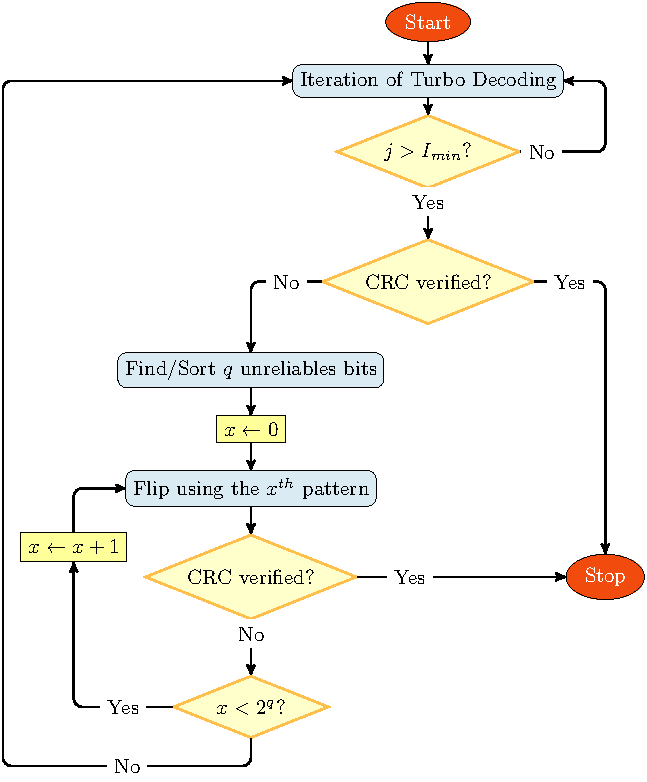
\includegraphics[width=\textwidth]{fig/flow/fc0.pdf}}
      \only<2>{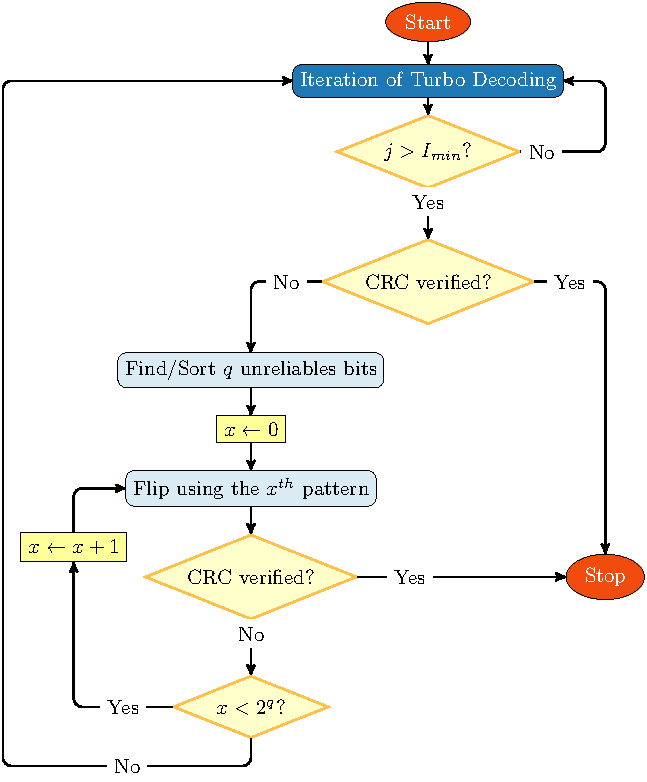
\includegraphics[width=\textwidth]{fig/flow/fc_tdec.pdf}}
      \only<3>{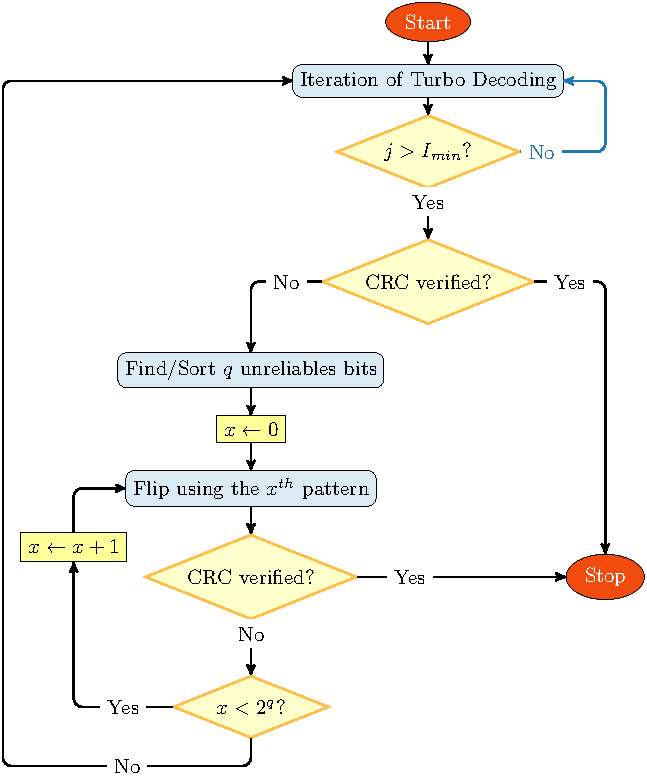
\includegraphics[width=\textwidth]{fig/flow/fc_reit.pdf}}
      \only<4>{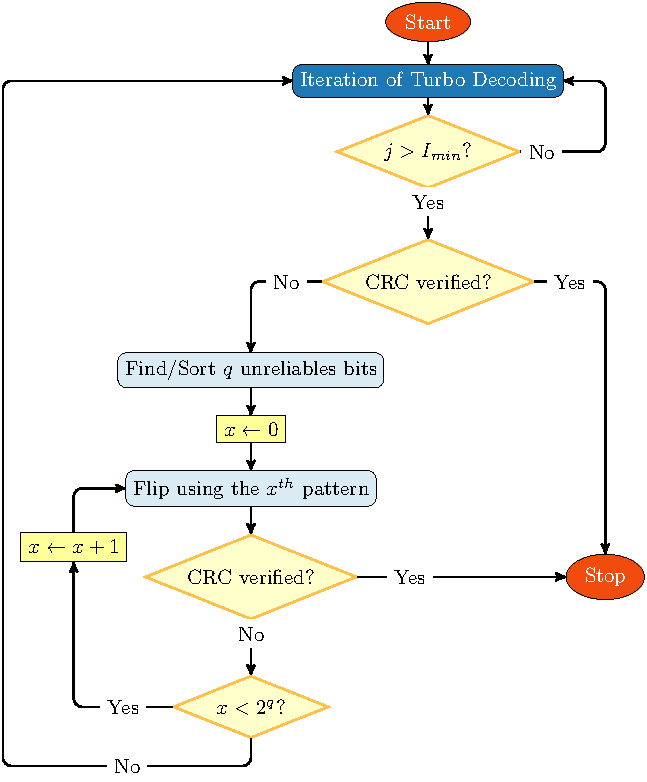
\includegraphics[width=\textwidth]{fig/flow/fc_tdec.pdf}}
      \only<5>{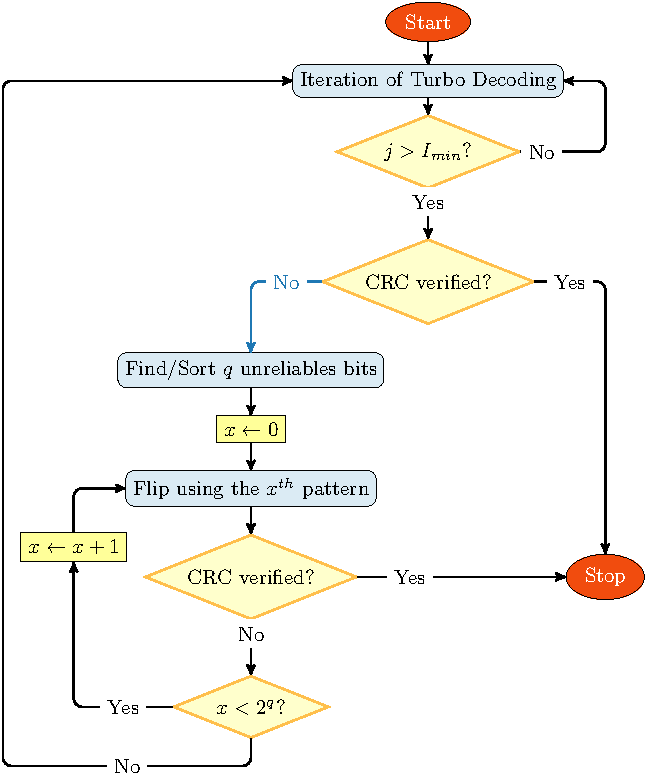
\includegraphics[width=\textwidth]{fig/flow/fc_nocrc.pdf}}
      \only<6>{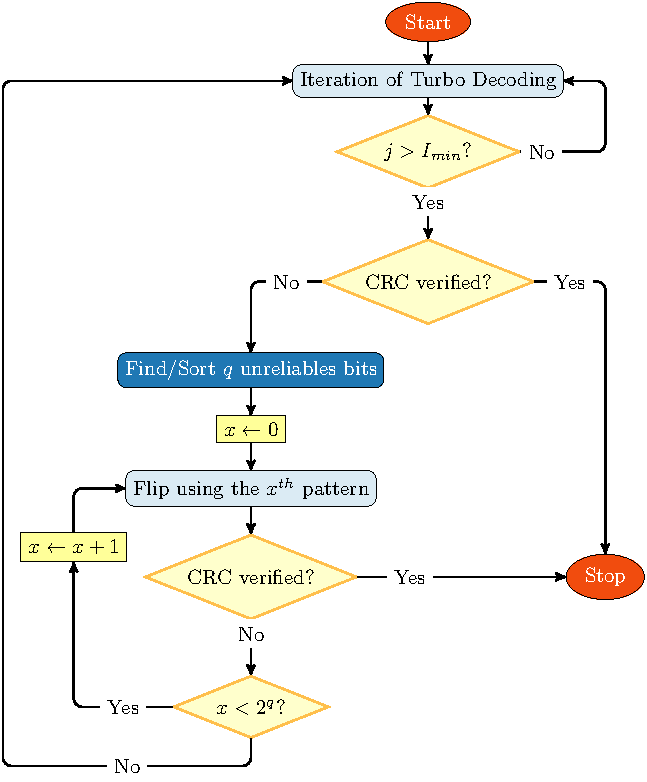
\includegraphics[width=\textwidth]{fig/flow/fc_find.pdf}}
      \only<7>{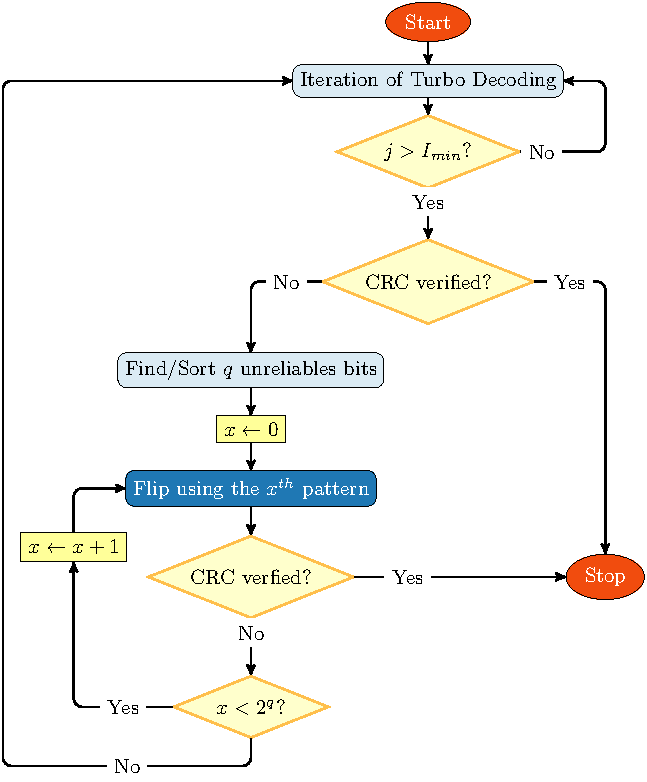
\includegraphics[width=\textwidth]{fig/flow/fc_flip.pdf}}
      \only<8>{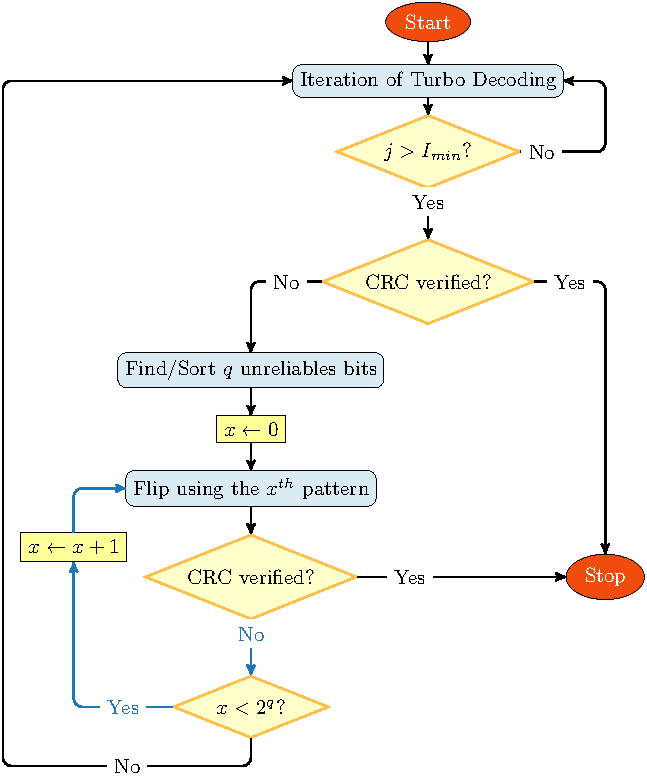
\includegraphics[width=\textwidth]{fig/flow/fc_flip2.pdf}}
      \only<9>{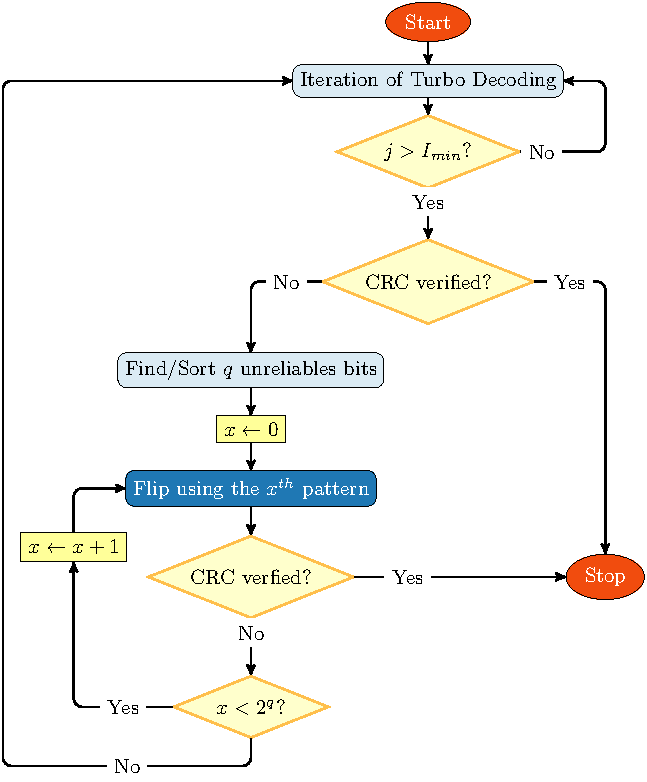
\includegraphics[width=\textwidth]{fig/flow/fc_flip.pdf}}
      \only<10>{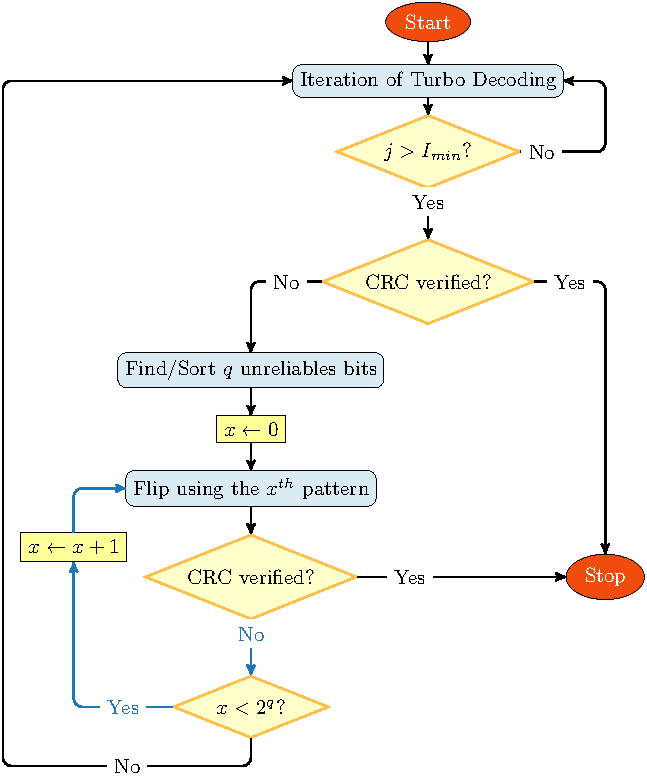
\includegraphics[width=\textwidth]{fig/flow/fc_flip2.pdf}}
      \only<11>{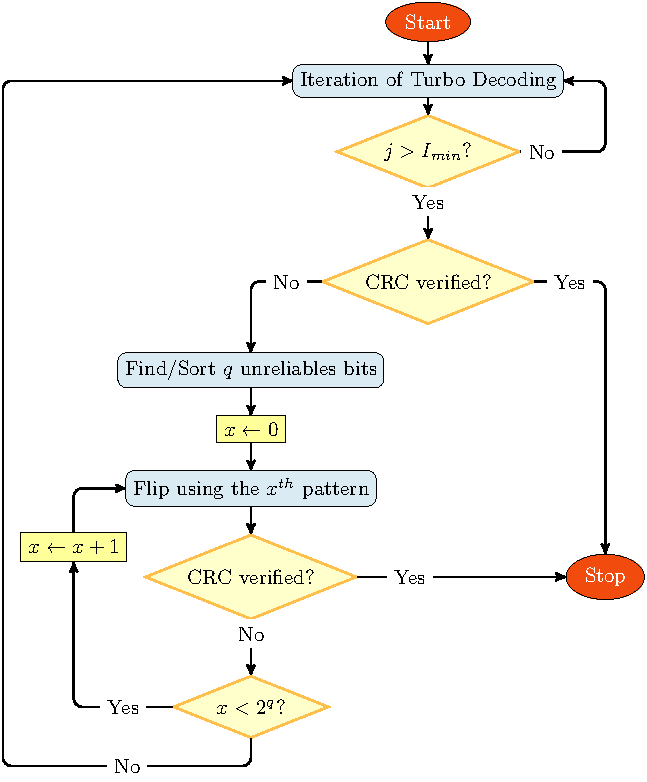
\includegraphics[width=\textwidth]{fig/flow/fc0.pdf}}
    \end{column}%
    \hfill%
    \begin{column}{.48\textwidth}
      \begin{center}
        \uncover<5->{
          \resizebox{\linewidth}{!}{
            \begin{tabular}{rllllllllll}
              & \multicolumn{7}{|c|}{\textit{input}} & \multicolumn{2}{|c|}{\textit{crc}} \\
              \toprule
              $\mathbf{\hat{d}}$ & \textcolor{Paired-5}{\textbf{0}}    & 1   & 1                                   & 0   & 1   & \textcolor{Paired-5}{\textbf{0}}    & 0   & 1   & 0   \\
              $\Delta$           & \only<6-9>{\cellcolor{Paired-6}}1.2 & 3.5 & \only<6-9>{\cellcolor{Paired-6}}0.2 & 4.2 & 5.1 & \only<6-9>{\cellcolor{Paired-6}}0.3 & 2.8 & 1.7 & 3.5 \\
              \bottomrule
            \end{tabular}}  }
      \end{center}
      \only<6->{{\small$q = 3$ positions are identified:}\resizebox{.31\linewidth}{!}{\begin{tabular}{ccc} 
        $k_2$ & $k_5$ & $k_0$ \\
        \end{tabular}}\\\vspace*{.2cm}}
      \only<7->{
        {\small$2^q - 1= 7$ candidate words are generated :}\\\vspace*{.2cm}
        \resizebox{\linewidth}{!}{\vspace*{.2cm}
          \begin{tabular}{rllllllllll}
            \toprule
            $\mathbf{d_1}$                                          & 0 ~~                                 & 1 ~~ & \only<7-10>{\cellcolor{Paired-4}}{0} ~~ & 0 ~~ & 1 ~~ & 0 ~~                                 & 0 ~~ & 1 ~~ & 0  \\
            \only<8->{$\mathbf{d_2}$                                & 0 ~~                                 & 1 ~~ & 1 ~~                                  & 0 ~~ & 1 ~~ & \only<8-10>{\cellcolor{Paired-4}}{1}   & 0 ~~ & 1 ~~ & 0} \\
            \only<9->{$\mathbf{d_3}$                                & \only<8-10>{\cellcolor{Paired-4}}{1} ~~ & 1 ~~ & 1 ~~                                  & 0 ~~ & 1 ~~ & 0 ~~                                 & 0 ~~ & 1 ~~ & 0} \\
            \only<10->{$\mathbf{d_4}$                                & 0 ~~                                 & 1 ~~ & \only<8-10>{\cellcolor{Paired-4}}{0} ~~  & 0 ~~ & 1 ~~ & \only<8-10>{\cellcolor{Paired-4}}{1} ~~ & 0 ~~ & 1 ~~ & 0} \\
            \only<10->{$\mathbf{d_5}$                                & \only<8-10>{\cellcolor{Paired-4}}{1} ~~ & 1 ~~ & \only<8-10>{\cellcolor{Paired-4}}{0} ~~  & 0 ~~ & 1 ~~ & 0 ~~                                 & 0 ~~ & 1 ~~ & 0} \\
            \only<10->{\only<11>{\cellcolor{Paired-3}}$\mathbf{d_6}$ & \only<8-10>{\cellcolor{Paired-4}}{1} ~~ & 1 ~~ & 1 ~~                                  & 0 ~~ & 1 ~~ & \only<8-10>{\cellcolor{Paired-4}}{1} ~~ & 0 ~~ & 1 ~~ & 0} \\
            \only<10->{$\mathbf{d_7}$                                & \only<8-10>{\cellcolor{Paired-4}}{1} ~~ & 1 ~~ & \only<8-10>{\cellcolor{Paired-4}}{0} ~~  & 0 ~~ & 1 ~~ & \only<8-10>{\cellcolor{Paired-4}}{1} ~~ & 0 ~~ & 1 ~~ & 0} \\
            \bottomrule
          \end{tabular}}\\\vspace*{.2cm}}
      \only<11->{{\small} These words are verified thanks to the CRC}
    \end{column}%
  \end{columns}
\end{frame}

\begin{frame}[c]{Performances de décodage}
\begin{center}
\begin{tikzpicture}
    \begin{semilogyaxis}[footnotesize, width=0.95\linewidth, height=0.6\linewidth,    
            xmin=0, xmax=3, xtick={0,0.5,...,3},
            %ymin=2e-6,  ymax=0.11,
            xlabel=$E_b/N_0 \text{(dB)}$, ylabel=FER,  grid=both, grid style={gray!30},
        tick align=outside, tickpos=left, %legend style={at={(0.5,-0.2)},anchor=north}]
        legend pos=north east]
        \addplot[mark=o,Paired-5, semithick]  table [x=SNR, y=FSF] {../main/ch3_fig/fnc/lte/dat/528};
        \addplot[mark=o,Paired-1, semithick]  table [x=SNR, y=FSF] {../main/ch3_fig/fnc/lte/dat/1024};
        \addplot[mark=o,Paired-3, semithick]  table [x=SNR, y=FSF] {../main/ch3_fig/fnc/lte/dat/2048};
        \addplot[mark=o,Paired-7, semithick]  table [x=SNR, y=FSF] {../main/ch3_fig/fnc/lte/dat/6144};
        \addplot[mark=o,Paired-5!50!Paired-6, semithick, dashed, mark options={solid}]  table [x=SNR, y=FER] {../main/ch3_fig/fnc/lte/dat/528};
        \addplot[mark=o,Paired-1!50!Paired-2, semithick, dashed, mark options={solid}]  table [x=SNR, y=FER] {../main/ch3_fig/fnc/lte/dat/1024};
        \addplot[mark=o,Paired-3!50!Paired-4, semithick, dashed, mark options={solid}]  table [x=SNR, y=FER] {../main/ch3_fig/fnc/lte/dat/2048};
        \addplot[mark=o,Paired-7!50!Paired-8, semithick, dashed, mark options={solid}, restrict x to domain=0.4:1.4]  table [x=SNR, y=FER] {../main/ch3_fig/fnc/lte/dat/6144};

        \legend{K=528, K=1024, K=2048, K=6144} 
         
    \end{semilogyaxis}
\end{tikzpicture}  
\end{center}
\vspace*{-3ex}
\captionof{figure}{Comparaison de performances de décodages entre EML-MAP et FNC. Standard LTE, K=528, 1024, 2048 et 6144. R=1/3.
  Décodeurs itérant jusqu'à 8 fois}
\end{frame}

\begin{frame}[c]{Turbo codes doubles binaires - Identification symboles}
\begin{itemize}\setlength\itemsep{2em}
  \item Dans le cas des TC double binaires, l'identification des positions les moins fiables correspond à un symbole
  \item Une transposition directe de l'algorithme binaire impliquerait alors une génération de $4^q$ mots candidats
  \item Or, par une approche statistique il apparaît que dans $96\%$ des cas, le symbole émis correspond au deuxième plus probable ($S_{m_y}$)
\end{itemize}
\vspace*{1em}
{\color{bleuUni}\Large\MVRightarrow} Mémorisation des 2 symboles les plus probables et génération de $2^q$ mots candidats
\end{frame}

\begin{frame}[c]{Turbo codes doubles binaires - Explication schématique}
  Comme avant ? ou ce n'est pas la peine ?
\end{frame}

\begin{frame}[c]{PTurbo codes doubles binaires - Performances de décodage}
  PROBLEME CRC LOULALILALOU\\
  À remplir avec occigen 

\end{frame}

\begin{frame}[c]{Comparaison état de l'art}
  Pas réellement bien fait dans le manuscrit...
\end{frame}


%%%%%%%%%%%%%%%%%%%%%%%%%%%%%%%%%%%%%%%%%%%%%%%%%%%%%%%%%%%%%%%%%%%%%%%%%%%%%%%%
\section[Architecture matérielle]{Architecture matérielle de correction des erreurs résiduelles}
%%%%%%%%%%%%%%%%%%%%%%%%%%%%%%%%%%%%%%%%
\subsection{Implantation matérielle de turbo décodeurs}
\begin{frame}[c]{Introduction}
\begin{itemize}\setlength\itemsep{1em}
  \item Interfacer l'algorithme avec un turbo décodeur
  \item Études préalables : 
  \begin{itemize}
    \item Architectures matérielles de turbo décodeurs
    \item Influence des paramètres de l'algorithme FNC sur
    \begin{itemize}
      \item Complexité calculatoire
      \item Performances de décodage
    \end{itemize}
  \end{itemize}
  \item Dans le cas binaire uniquement
\end{itemize}
\end{frame}

\begin{frame}[c]{Schéma d'une architecture de turbo code séquentiel}
\begin{center}
  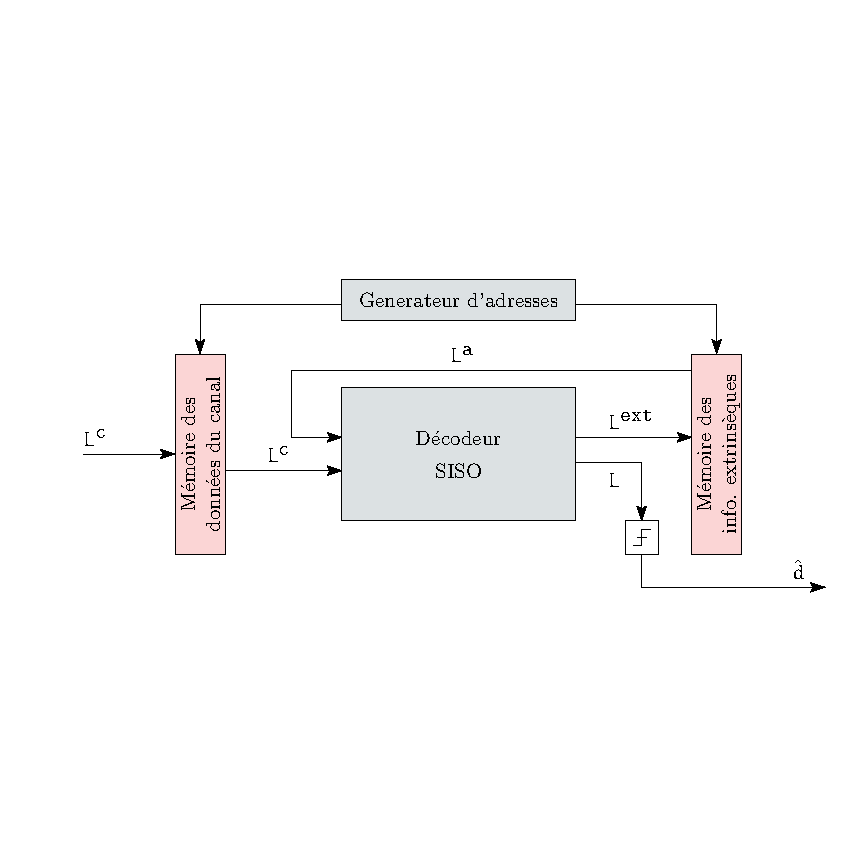
\includegraphics[width=.8\columnwidth]{../main/ch4_fig/ipe/serial.pdf}
\end{center}
\captionof{figure}{Principe du turbo décodage séquentiel.}
\end{frame}

\begin{frame}[c]{Les différents ordonnancements des calculs}
\only<1>{\begin{itemize}\setlength\itemsep{1em}
  \item BCJR : parcours aller retour dans le treillis
  \item Étapes des calculs :\\
   \begin{itemize}\setlength\itemsep{2ex}
     \item Métriques de branches ($\gamma$)
     \begin{itemize}
       \item Métriques de nœuds aller ($\alpha$)
       \item Métriques de nœuds retour ($\beta$)
     \end{itemize}
    \qquad \qquad {\color{bleuUni}\Large\MVRightarrow} Informations \textit{a posteriori} ($L^\text{a}$)
   \end{itemize}
\end{itemize}}

\only<2>{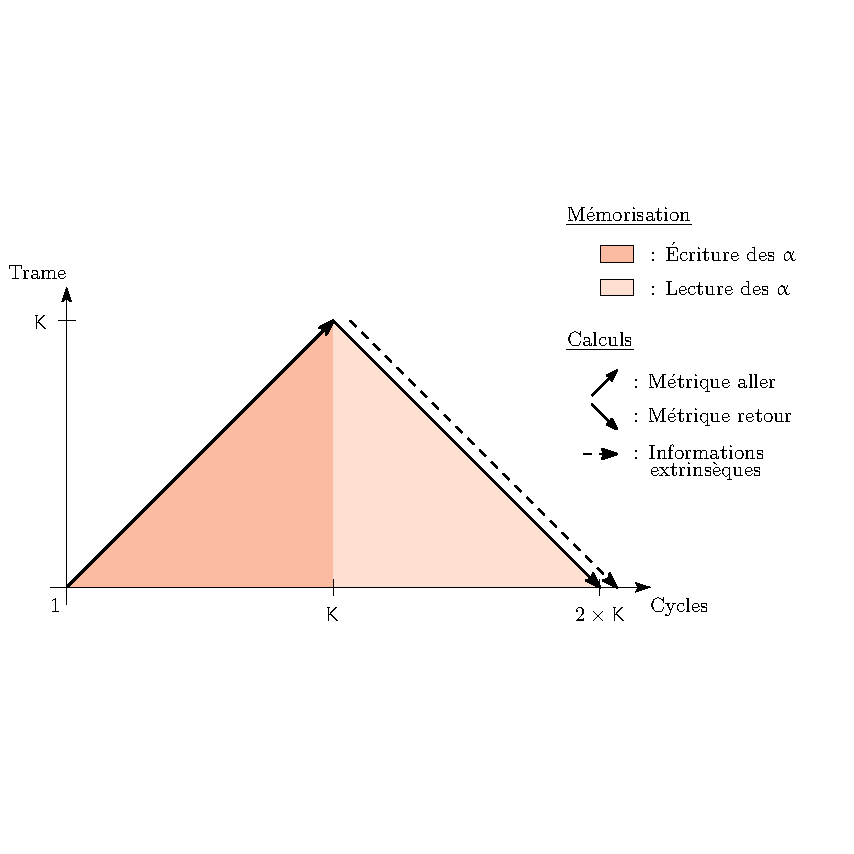
\includegraphics[width=.8\columnwidth, right]{../main/ch4_fig/ipe/FB+LEG_2.pdf}
        \captionof{figure}{Ordonnancement BCJR Aller-Retour.}}

\only<3>{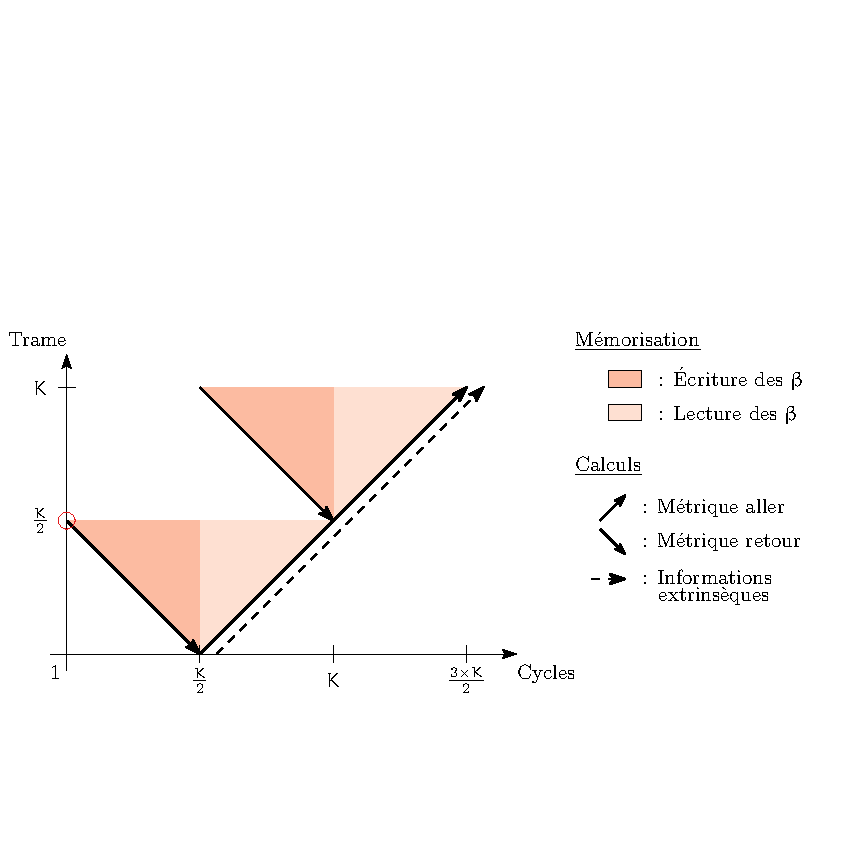
\includegraphics[width=.8\columnwidth, right]{../main/ch4_fig/ipe/BF_SW+LEG.pdf}
         \captionof{figure}{Ordonnancement BCJR Retour-Aller avec fenêtre glissante, W=2.}}

\only<4>{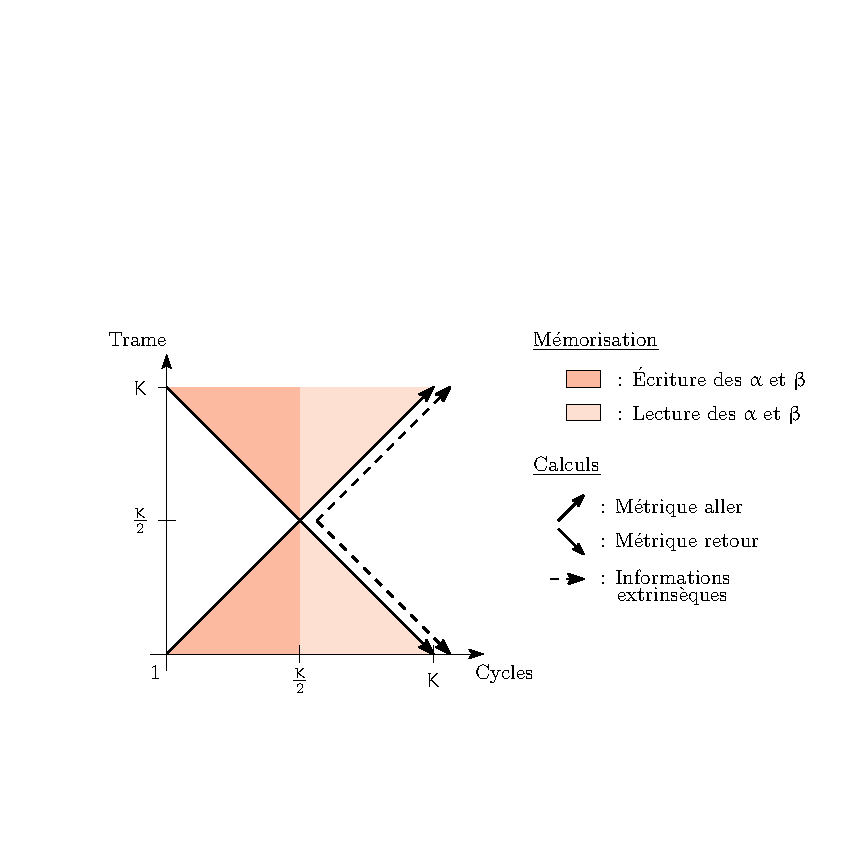
\includegraphics[width=.8\columnwidth, right]{../main/ch4_fig/ipe/BFLY+LEG.pdf}
         \captionof{figure}{Ordonnancement BCJR Butterfly.}}

\only<5>{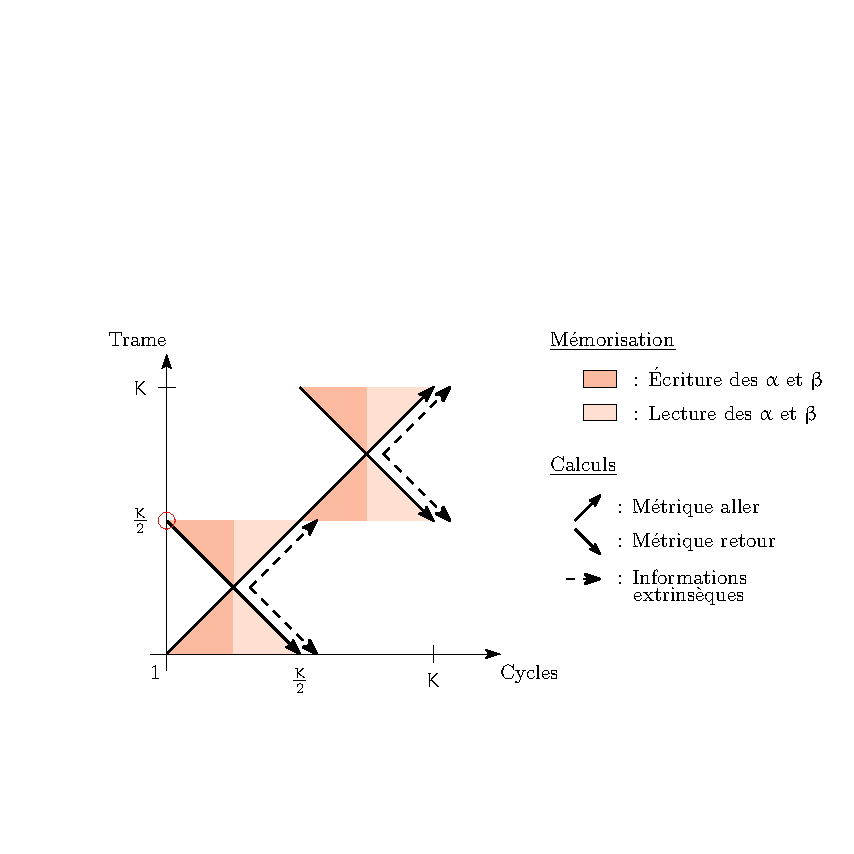
\includegraphics[width=.8\columnwidth, right]{../main/ch4_fig/ipe/BFLY_SW+LEG.pdf}
          \captionof{figure}{Ordonnancement BCJR Butterfly avec fenêtre glissante.}}

\only<6>{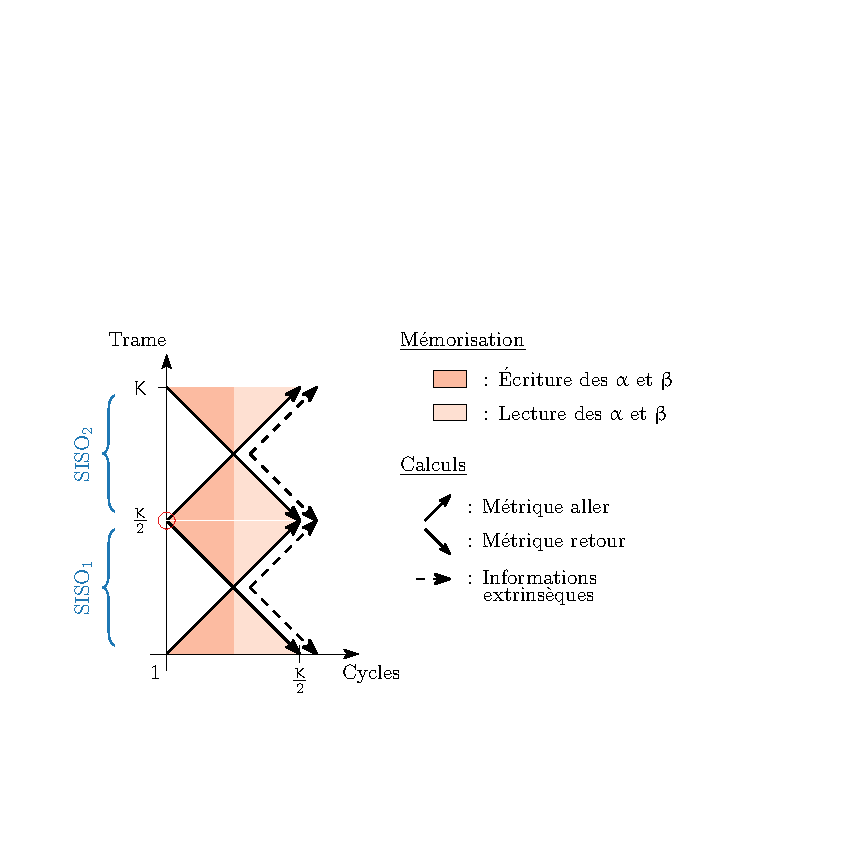
\includegraphics[width=.8\columnwidth, right]{../main/ch4_fig/ipe/BFLY_SB+LEG.pdf}
         \captionof{figure}{Ordonnancement BCJR Butterfly en parallèle.}}

\only<7>{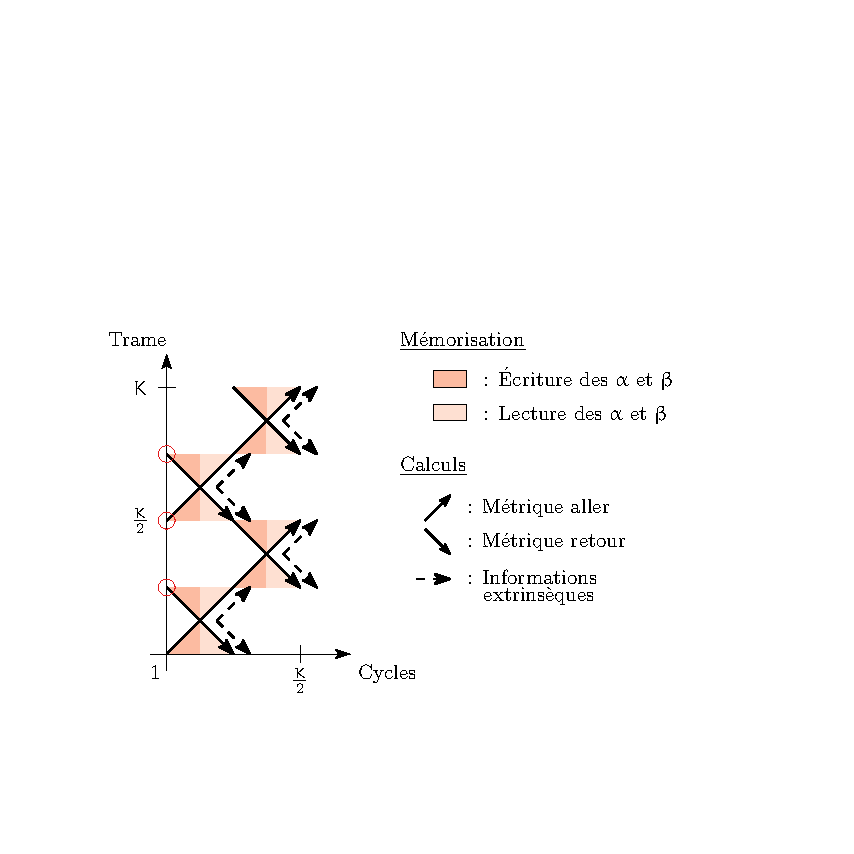
\includegraphics[width=.8\columnwidth, right]{../main/ch4_fig/ipe/BFLY_SB_SW+LEG.pdf}
         \captionof{figure}{Ordonnancement BCJR Butterfly avec fenêtre glissante en parallèle.}}

\end{frame}

\begin{frame}[c]{Ordonnancement retenu}
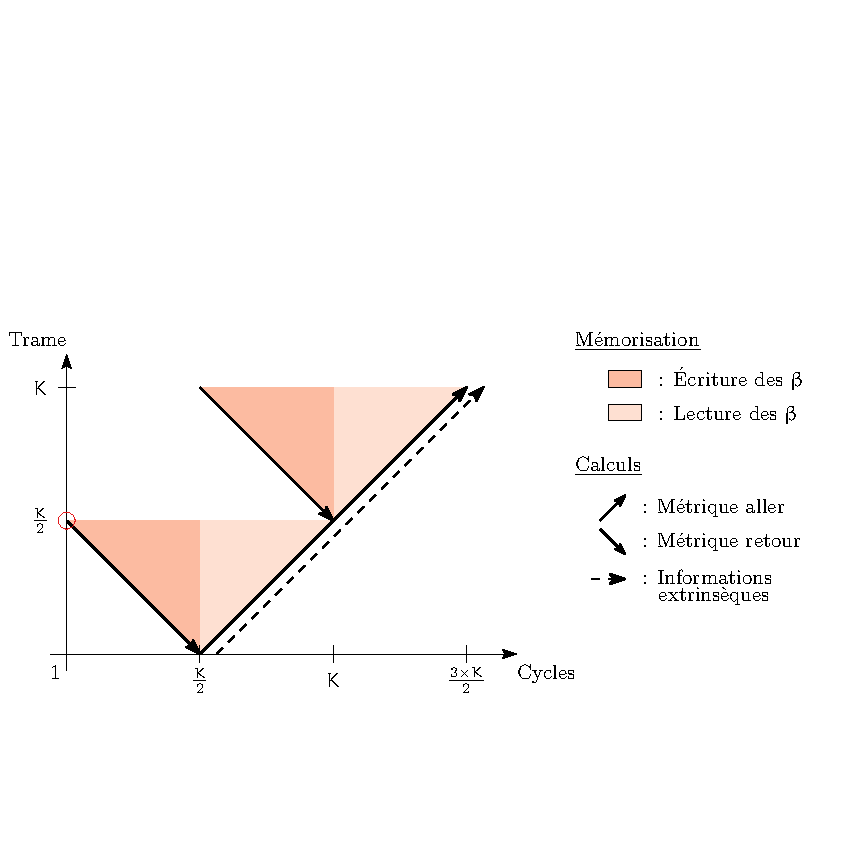
\includegraphics[width=.8\columnwidth, right]{../main/ch4_fig/ipe/BF_SW+LEG.pdf}
  \captionof{figure}{Ordonnancement BCJR Retour-Aller avec fenêtre glissante, W=2 (BF-SW).}
\vspace*{2ex}
  \resizebox{1\textwidth}{!}{
\begin{tabular}{rllll}
\toprule
Ordonnancement      & \begin{tabular}[c]{@{}l@{}}Durée d'une \\ demi-itération\end{tabular} & \begin{tabular}[c]{@{}l@{}}Durée d'une \\ itération\end{tabular} & \begin{tabular}[c]{@{}l@{}}Durée de la transmission \\ d'informations \textit{a posteriori} \end{tabular} & \begin{tabular}[c]{@{}l@{}}Nombre d'informations \\\textit{a posteriori} simultanées\end{tabular}     \\
\cmidrule(r){1-1}   \cmidrule(l){2-2}        \cmidrule(l){3-3} \cmidrule(l){4-4}                  \cmidrule(l){5-5}    
BF-SW (W)           & $K + \ddfrac{K}{W}$  & $2\times(K + \ddfrac{K}{W})$ & $K$                    & 1               \\
\bottomrule
\end{tabular}}
\end{frame}

%%%%%%%%%%%%%%%%%%%%%%%%%%%%%%%%%%%%%%%%
\subsection{Les paramètres de l'algorithme FNC}
\begin{frame}[c]{Intro}
\begin{itemize}
  \item L'algorithme FNC est ajustable en fonction de plusieurs paramètres
  \item Double impact : complexité calculatoire et performances de décodage
  \item Objectif : Réduire la complexité calculatoire et présenter la dégradation de performances associés
  \item Trois axes : 
  \begin{itemize}
    \item Nombre d'applications du processus FNC par trame
    \item Nombre de mots candidats considérés
    \item Quantification des informations internes au processus FNC
  \end{itemize}
\end{itemize}
\end{frame}

\begin{frame}[c]{Processus itératif}
  \includegraphics[width=\textwidth, center]{../main/ch4_fig/final/tikz_last/fnc10_minX.pdf}
\end{frame}

\begin{frame}[c]{Nombre de mots candidats}
Animation
\end{frame}

\begin{frame}[c]{Quantification}
Dessin \\
Tableau
\end{frame}

%%%%%%%%%%%%%%%%%%%%%%%%%%%%%%%%%%%%%%%%
\subsection{Implantation matérielle de l'algorithme FNC}
\begin{frame}[c]{Principe et ordonnancement}
DASIP
\end{frame}

\begin{frame}[c]{Les différents blocs}
Animation DASIP
\end{frame}

\begin{frame}[c]{Résultats d'implantations}
Dessin \\
Tableau
\end{frame}

%%%%%%%%%%%%%%%%%%%%%%%%%%%%%%%%%%%%%%%%%%%%%%%%%%%%%%%%%%%%%%%%%%%%%%%%%%%%%%%%
\section[Conclusions]{Conclusions et perspectives}

\begin{frame}[c]{Conclusions}
TODO
\end{frame}

\begin{frame}[c]{Perspectives}
TODO
\end{frame}

\begin{frame}[c]{Merci}
\begin{center}
Merci pour votre attention !
\end{center}
\end{frame}

\end{document}
